%-------------------------------------------------------------------------------
% This file provides a skeleton ATLAS note.
\pdfinclusioncopyfonts=1
% This command may be needed in order to get \ell in PDF plots to appear. Found in
% https://tex.stackexchange.com/questions/322010/pdflatex-glyph-undefined-symbols-disappear-from-included-pdf
%-------------------------------------------------------------------------------
% Specify where ATLAS LaTeX style files can be found.
\RequirePackage{latex/atlaslatexpath}
% You can comment out the above line if the files are in a central location, e.g. $HOME/texmf.
%-------------------------------------------------------------------------------
\documentclass[NOTE, REPORT=true, atlasdraft=true, UKenglish]{atlasdoc}
% The language of the document must be set: usually UKenglish or USenglish.
% british and american also work!
% Commonly used options:
%  atlasdraft=true|false This document is an ATLAS draft.
%  NOTE                  The document is an ATLAS note (draft).
%  REPORT=true|false     Use scrreprt|scrartcl as main class for document.
%  paper=a4|letter       Set paper size to A4 (default) or letter.

%-------------------------------------------------------------------------------
% Extra packages:
\usepackage{atlaspackage}
% Commonly used options:
%  subfigure|subfig|subcaption  to use one of these packages for figures in figures.
%  minimal               Minimal set of packages.
%  default               Standard set of packages.
%  full                  Full set of packages.
%-------------------------------------------------------------------------------

% Adds multi-comment command:
\usepackage{verbatim}

% Style file with biblatex options for ATLAS documents.
\usepackage{atlasbiblatex}
% Commonly used options:
%  backref=true|false    Turn on or off back references in the bibliography.

% Package for creating list of authors and contributors to the analysis.
\usepackage{atlascontribute}

% Useful macros
\usepackage{atlasphysics}
% See doc/atlas_physics.pdf for a list of the defined symbols.
% Default options are:
%   true:  journal, misc, particle, unit, xref
%   false: BSM, hepparticle, hepprocess, hion, jetetmiss, math, process,
%          other, snippets
% See the package for details on the options.

% Macro to add to-do notes (for several authors). Uses the todonotes package.
% \ATLnote{JS}{Jane}{green!20}{green!50!black!60}
% add macros \JSnote and \JSinote for notes in the margin and inline.
% The first colour is for the body and the second for the border of the note.
% Set output=false in order not to print out the notes.
% Set shift=false to avoid adjustment of margins.
% Check for notes still left by commenting out the package in the final version of the note.
\usepackage[output=true, shift=true]{atlastodo}

% Files with references for use with biblatex.
% Note that biber gives an error if it finds empty bib files.
\addbibresource{ANA-HION-2025-03-INT1.bib}
\addbibresource{bib/ATLAS.bib}
\addbibresource{bib/CMS.bib}
\addbibresource{bib/ConfNotes.bib}
\addbibresource{bib/PubNotes.bib}

% Paths for figures - do not forget the / at the end of the directory name.
\graphicspath{{logos/}{figures/}}

% Add your own definitions here (file ANA-HION-2025-03-INT1-defs.sty).
\usepackage{ANA-HION-2025-03-INT1-defs}

%-------------------------------------------------------------------------------
% Generic document information.
%-------------------------------------------------------------------------------

% Title, abstract and document.
%-------------------------------------------------------------------------------
% This file contains the title, author and abstract.
% It also contains all relevant document numbers used for an ATLAS note.
%-------------------------------------------------------------------------------

% Title
\AtlasTitle{Charged particle $\RAA$ in $\OO$ and $\NeNe$ collisions at $\sqn=\qty{5.36}{TeV}$}

% Draft version:
% Should be 1.0 for the first circulation, and 2.0 for the second circulation.
% If given, adds draft version on front page, a 'DRAFT' box on top of each other page, 
% and line numbers.
% Comment or remove in final version.
\AtlasVersion{0.3}

% Abstract - % directly after { is important for correct indentation
\AtlasAbstract{The analysis investigates possible suppression or enhancement of inclusive charged hadron production in $\sqn=5.36$~TeV collisions of \OO and \NeNe compared to the \pp collisions at the same energy measured by the ATLAS detector at the LHC. The results are compared to theoretical predictions.}

% Author - this does not work with revtex (add it after \begin{document})
\author{The ATLAS Collaboration}

% Authors and list of contributors to the analysis
% \AtlasAuthorContributor also adds the name to the author list
% Include package latex/atlascontribute to use this
% Use authblk package if there are multiple authors, which is included by latex/atlascontribute
% \usepackage{authblk}
% Use the following 3 lines to have all institutes on one line
% \makeatletter
% \renewcommand\AB@affilsepx{, \protect\Affilfont}
% \makeatother
% \renewcommand\Authands{, } % avoid ``. and'' for last author
% \renewcommand\Affilfont{\itshape\small} % affiliation formatting
% \AtlasAuthorContributor{First AtlasAuthorContributor}{a}{Author's contribution.}
% \AtlasAuthorContributor{Second AtlasAuthorContributor}{b}{Author's contribution.}
% \AtlasAuthorContributor{Third AtlasAuthorContributor}{a}{Author's contribution.}
% \AtlasContributor{Fourth AtlasContributor}{Contribution to the analysis.}
% \author[a]{First Author}
% \author[a]{Second Author}
% \author[b]{Third Author}
% \affil[a]{One Institution}
% \affil[b]{Another Institution}


% If a special author list should be indicated via a link use the following code:
% Include the two lines below if you do not use atlasstyle:
% \usepackage[marginal,hang]{footmisc}
% \setlength{\footnotemargin}{0.5em}
% Use the following lines in all cases:
% \usepackage{authblk}
% \author{The ATLAS Collaboration%
% \thanks{The full author list can be found at:\newline
%   \url{https://atlas.web.cern.ch/Atlas/PUBNOTES/ATL-PHYS-PUB-2016-007/authorlist.pdf}}
% }

% ATLAS reference code, to help ATLAS members to locate the paper
\AtlasRefCode{ANA-HION-2025-03}

% ATLAS note number. Can be an COM, INT, PUB or CONF note
\AtlasNote{ANA-HION-2025-03-INT1}

% Author and title for the PDF file.
\hypersetup{pdftitle={ATLAS document},pdfauthor={The ATLAS Collaboration}}

%-------------------------------------------------------------------------------
% Content
%-------------------------------------------------------------------------------
\begin{document}

\maketitle

\tableofcontents

% List of contributors - print here or after the Bibliography.
% \PrintAtlasContribute{0.30}
% \clearpage

% List of to-do notes.
% \listoftodos

\chapter{Introduction}
\label{chap:intro}

The analysis aims to investigate possible suppression or enhancement of inclusive charged-hadron production in $\sqn=5.36$~TeV collisions of $\OO$ and $\NeNe$ using the ATLAS detector at the LHC in the form of a fast track analysis. The goal is to measure $\RAA$ up to its statistical limit, that is, given the short pilot $\OO$ run planned in July, will be limited to $\pT$ of 50 GeV inclusively in centrality. This reach is estimated based on the comparison to the reach of the $\RpPb$ measurement during the $\pPb$ pilot run (1~$\mu$b, \cite{pPb_pilot} taken at a comparable energy $\sqn=5.02$~TeV in 2012, the slope of the charge hadron spectrum \cite{chargedHadronATLAS}, and an expected factor of 1000 times higher collected luminosity as presented during the Corr\&Fluc subgroup meetings \cite{pt_reach_projection_1}. Analysis of the $\NeNe$ nuclear modification based on the results of neon ions colliding by the LHC shortly after oxygen is expected to have comparable or lesser data volume and follow the $\OO$ measurement. Therefore, it is not considered separately. 

The 425~\ipb of $\pp$ baseline data at the same per-nucleon energy was obtained by the ATLAS detector in 2024. These data, in principle, allow measuring charged hadron spectra to a much higher $\pT$, but that measurement has not been performed yet. As it has been proven by many previous works, measuring charged particle spectra up to intermediate momenta, like $\pT=50$~GeV and higher momenta~\cite{chargedHadronATLAS} requires significantly different approaches in the analysis and the amount of work. For that reason, and to provide a fast, yet precise measurement with ATLAS, the analysis strategy for this measurement was suggested as explained below. 

\section{Existing results and predictions}

Charged hadron spectra have been previously studied by ATLAS in $\pp$, $\pPb$, $\PbPb$, and $\XeXe$ at $\sqn=\qty{5.02}{\TeV}$ \cite{chargedHadronATLAS} as well as $\frac{d\nchar}{d\eta}$ in $\pPb$ at the same energy \cite{ATLAS:2015hkr} as a broader attempt to bridge the description of collisions of small systems and the peripheral collisions of large systems. $\OO$ and $\NeNe$ represent an intermediate system between $\pp$ and $\PbPb$, while the detector activity ought to resemble $\pPb$ collisions. Nuclear modification factor of the charged hadrons in the O+O collisions was studied by the STAR experiment at $\sqn = \qty{200}{\GeV}$. Preliminary results were shown at the QM25 \cite{star_roo_qm25}.

\section{Definition of variables}
Nuclear modification factor $R_{\mathrm{AB}}$ is generally defined as
\begin{equation}
    R_{\mathrm{AB}} = \sigma^{\mathrm{AB}}/(A\times B \times \sigma_{_{\mathrm{NN}}}),
\end{equation}
where $\sigma^{\mathrm{AB}}$ is a reaction cross section in ion-ion collisions, A and B are the atomic numbers of the colliding species, and $\sigma_{_{\mathrm{NN}}}$ is a nucleon-nucleon interaction cross section. For a symmetric system A=B, $R_{\mathrm{AB}}$ is denoted as $\RAA$. Since most of the measurements are using $\pp$ collisions as a baseline, $\sigma_{_{\mathrm{NN}}}$ is typically replaced by $\sigma_{\pp}$. Conventionally, a correction for the isospin differences resulting from $\sigma_{_{\mathrm{NN}}}\neq\sigma_{\pp}$ is not applied to the experimental results, unless it is specifically discussed. 

When $\RAA \sim 1$, the nuclear collision happens as the uncorrelated sum of nucleon-nucleon collisions. Indeed, for high-\pT probes without the color charge, such as Z and W bosons, the $\RAA$ is consistent with unity \cite{W_boson, Z_boson}. Conversely, the $\RAA$ deviates from unity for jets and charged hadrons as these probes are suppressed in the interactions with the quark-gluon plasma (QGP) created in the heavy ion collisions. The deviation is more significant in more central collisions \cite{jet_RAA}, where higher losses of color-charged probes are observed.
% the QGP is more dense and hot {\blue or just larger, thus increasing path length, how one distinguishes?}, causing higher losses of color-charged probes.

Furthermore, the measurements are usually performed differentially in kinematic variables of the produced particles. Therefore, a commonly used definition is written as: 
\begin{equation}
% \RAA = \frac{1}{\avgTAA}\frac{(1/N^{\text{AA}}_\text{evt})\dif^2 N^{\text{AA}} / \dif \pT\dif\eta }{\dif^2\sigma^{\pp} / \dif \pT\dif\eta}, 
  %  \quad 
    \RAA = \frac{1}{A^2}\frac{\dd^2 \sigma^{\text{AA}}/\dd\pT\dd\eta }{\dd^2\sigma^{\pp} / \dd\pT\dd\eta},
\end{equation}
Given we will have access only to the $\pprefSample$ luminosity $\mathcal{L}_{pp}$, but not to the \OO one, the $\RAA$ can be calculated using the $\RAA$ the nuclear thickness function $\TAA$ (sometimes called “per collision luminosity”)
\begin{equation}
    \RAA = 
    \frac{\mathcal{L}_{pp}}{\TAA}
    \frac{1}{N^{\mathrm{AA}}_{\mathrm{evt}}}
    \frac{\dd^2 n^{\mathrm{AA}}_{\mathrm{ch}}\dd\pT\dd\eta}
         {\dd^2 n^{\pp}_{\mathrm{ch}}/\dd\pT\dd\eta},
    \label{eqn:RAA_measurable}
\end{equation}
where $N^{\mathrm{AA}}_{\mathrm{evt}}$ is the number of analyzed collision events in the \OO samples, and $n_{\mathrm{ch}}$ is the number of charged particles (hadrons) in either $\pprefSample$ or \OO sample. 

\section{Analysis strategy}
The analysis strategy chosen for this measurement aims to produce the most accurate and fastest results using the new data. We anticipate that the interest in this measurement in the HI community will be very high; therefore, providing a fast measurement has its value. We start from the following considerations.
\begin{itemize}
\item[$\cdot$] the full statistics of the \OO run will be sufficient to measure \RAA in the range up to $\pT=50$~GeV.
\item[$\cdot$] the \pp reference, obtained last year, was taken under similar detector conditions as the upcoming run and has significantly larger statistics.
\item[$\cdot$] given the large statistics accumulated in 2024 data, working out the charged hadron spectrum in \pp is a significant effort that would require resources comparable to measurements of the \RAA in \OO system. Therefore, we suggest not publishing the fully corrected spectra not in \pp and not in \OO, but entirely focusing on the \RAA.
\item[$\cdot$] the measurements of the \RAA is typically done differentially in \pT, in rapidity and in interval of centrality. Since the \OO is a symmetric system, the run statistics is limited and $\eta$-dependencies are not expected to be strong, we will measure the results integrated over the detector coverage, i.e., in $|\eta|<2.5$.
\item[$\cdot$] The measurement to be performed in this analysis will not be done in different intervals of centrality, but will be averaged over the minbias sample. This decision follows two goals: the first is a desire to produce a fast result. At the same time, centrality association, especially in a small system, is not a trivial procedure and requires a systematic uncertainty coming from the association procedure, which may become a leading uncertainty of a measurement. Since the anticipated deviation of the \RAA in this measurement at most 25 \% at the low-\pT edge and getting closer to 1 as the \pT grows (see Figure~\ref{fig:RAA_prediction}), we prefer avoiding additional uncertainty coming from working out centrality intervals.
\end{itemize}

Given these consideration, the equation~\eqref{eqn:RAA_measurable} can be written as
\begin{equation}
    \RAA = 
    \frac{\mathcal{L}_{pp}}{\avgTAA}
    \frac{1}{N^{\mathrm{AA}}_{\mathrm{evt}}}
    \frac{\dd n^{\mathrm{AA}}_{\mathrm{trk}}\dd\pT}
         {\dd n^{\pp}_{\mathrm{trk}}/\dd\pT}C(\pT)
    \label{eqn:RAA_final}
\end{equation}
where \avgTAA is the number of \TAA in the analysed interval of centralities -- minbias sample, $n_{\mathrm{trk}}$ is the number of tracks reconstructed in the detector and passed the selection criteria, and $C(\pT)$ is a composite factor related to the difference in detector conditions between \pp and $\text{AA}$ data-taking conditions. Analyzing the minimum bias sample, we hope that \avgTAA will be very close to the \TAA that can be extracted from the Glauber model, and given that the conditions of the 2024 and 2025 data taking and processing are close to each other, the $C(\pT)$ factor is going to be close to unity. Thus, the uncertainties that are expected in the measurements of \RAA in the proposed analysis strategy will come from \textit{i)} statistics of the \OO sample, \textit{ii)} $C(\pT)$ \textit{iii)} uncertainty on the $\mathcal{L}_{pp}$, \textit{iv)} \TAA determination from the model, and \textit{v)}
measurements of $N_{\mathrm{evt}}$ in \OO, detailed in Chapter~\ref{chap:corr}. The last two factors do not affect the \pT dependence of the \RAA.

%Analysis methods (track quality and track-to-vertex matching selections) are chosen to facilitate measurement in the low-\pT reach, while allowing quick analysis. The analysis pace is also supported by the definition of the \RAA based on \Ncoll and correction factor $C$, avoiding waiting for luminosity and detailed studies of track reconstruction efficiencies and pile-up removal. Finally, most of the corrections and systematics, which would be needed for measuring charged hadron spectra separately in $\ppref$ and \OO neglect each other in \RAA measurement. 




%\chapter{ATLAS detector}\label{chap:ATLAS}
{\red Maybe it is wise to write some relevant info on detector subsystems used here to later copy-paste into the paper?}
\section{General information}
\section{Trigger system}
\section{Inner Detector}
\section{Calorimeters}
\chapter{Datasets and simulations}
\label{chap:dataset}
\section{Datasets}
In the $\pprefSample$ same both MinBias (MB) and Main streams containing MB and jet triggers are used to extend the kinematic reach, matching the kinematic reach of \OO spectrum and bringing in as small statistical error as possible. In \OO and \NeNe, all triggers were present in the MB stream, and the full available statistic is analyzed. The triggers used to select studied events were used to maximize the statistics and are listed in Table~\ref{tab:comb}. The data analyzed were reconstructed in the HIP reconstruction mode. 

\begin{table}[!h]
\begin{center}
\renewcommand{\arraystretch}{1.5} % Increase the height of all rows
\setlength{\tabcolsep}{2.5pt} % Adjust this value to shrink or expand column spacing
\begin{tabular}{cccccc}
System & $\sqn\ [\TeV]$ & Stream & Trigger & Release \\ \hline
$\pprefSample$  & 5.36 & MinBias & $\pprefMBtrig$ & f1529\_m2259  \\
$\pprefSample$  & 5.36 & Main & HLT\_j30a\_L1jTE20 & f1529\_m2259  \\
$\pprefSample$  & 5.36 & Main & HLT\_j40\_L1jJ40 & f1529\_m2259  \\
$\pprefSample$  & 5.36 & Main & HLT\_j60\_L1jJ50 & f1529\_m2259  \\
$\pprefSample$  & 5.36 & Main & HLT\_j85\_L1jJ50 & f1529\_m2259  \\
$\pprefSample$  & 5.36 & Main & HLT\_j100\_L1jJ60 & f1529\_m2259  \\
$\OO$  & 5.36 & MinBias & HLT\_mb\_sptrk\_L1TRT\_FILLED & f1606\_m2272  \\
$\OO$  & 5.36 & MinBias & HLT\_j20\_ionp\_L1jJ10 & f1606\_m2272  \\
$\OO$  & 5.36 & MinBias & HLT\_j40\_ionp\_L1jJ20 & f1606\_m2272  \\
$\NeNe$  & 5.36 & MinBias & HLT\_mb\_sptrk\_L1TRT\_FILLED & f1606\_m2272  \\
$\NeNe$  & 5.36 & MinBias & HLT\_j20\_ionp\_L1jJ10 & f1606\_m2272  \\
$\NeNe$  & 5.36 & MinBias & HLT\_j40\_ionp\_L1jJ20 & f1606\_m2272  \\
\end{tabular}
\end{center}
\caption{Data samples}
\label{tab:comb}
\end{table}

% waiting for Angantyr

\section{MC samples}
To obtain the correction factor $C^{pp/\text{AA}}(p_T, \eta)$ and for the supporting studies of corrections and cuts, Angantyr samples $\pprefSample$ and pre-\OO run conditions were generated.

The additional MCs to be used in the supporting studies were Pythia 8.308 dijet samples with $\pprefSample$ conditions and $\sqn$ = 5.36~TeV, they are listed in Table \ref{tab:pythia}.
{\red will need updates after studies + list O+O samples to be used}
\begin{table}[!h]
\begin{center}
\renewcommand{\arraystretch}{1.5} % Increase the height of all rows
\setlength{\tabcolsep}{2.5pt} % Adjust this value to shrink or expand column spacing
\begin{tabular}{p{0.3\linewidth} p{0.3\linewidth}p{0.3\linewidth}}
\text{\centering $\mathrm{N_{evt}} [10^6]$} & \text{\centering $\sigma [\inb]$} & \text{\centering $\epsilon_{\mathrm{fil}}$} \\ \hline 
\multicolumn{3}{c}{mc23\_5p36TeV.801165.Py8EG\_A14NNPDF23LO\_jj\_JZ0.recon.AOD.e8551\_s4521\_s4483\_r16578} \\
15 & 6.8260 $\cdot 10^7$ & 9.9342 $\cdot 10^{-1}$ \\ \hline
\multicolumn{3}{c}
{mc23\_5p36TeV.801166.Py8EG\_A14NNPDF23LO\_jj\_JZ1.recon.AOD.e8551\_s4521\_s4483\_r16578} \\
15 & 3.3878 $\cdot 10^7$ & 1.8563 $\cdot 10^{-2}$ \\ \hline
\multicolumn{3}{c}
{mc23\_5p36TeV.801167.Py8EG\_A14NNPDF23LO\_jj\_JZ2.recon.AOD.e8551\_s4521\_s4483\_r16578} \\
15 & 7.0547 $\cdot 10^5$ & 6.5344 $\cdot 10^{-3}$ \\ \hline
\multicolumn{3}{c}
{mc23\_5p36TeV.801168.Py8EG\_A14NNPDF23LO\_jj\_JZ3.recon.AOD.e8551\_s4521\_s4483\_r16578} \\
15 & 5.3640 $\cdot 10^3$ & 7.560 $\cdot 10^{-3}$ \\ \hline
\multicolumn{3}{c}
{mc23\_5p36TeV.801169.Py8EG\_A14NNPDF23LO\_jj\_JZ4.recon.AOD.e8551\_s4521\_s4483\_r16578} \\
9.5 & 3.1658 $\cdot 10^1$ & 6.9140 $\cdot 10^{-3}$ \\ \hline
\multicolumn{3}{c}
{mc23\_5p36TeV.801170.Py8EG\_A14NNPDF23LO\_jj\_JZ5.recon.AOD.e8551\_s4521\_s4483\_r16578} \\
9.5 & 2.8793 $\cdot 10^{-1}$ & 4.3236 $\cdot 10^{-3}$ \\ 
\end{tabular}
\end{center}
\caption{Pythia 8.308 dijet samples at 5.36~TeV with $\pprefSample$ conditions}
\label{tab:pythia}
\end{table}

\blue{} Add the new dijet samples \black{}

 \begin{comment}
 were generated in three groups. The first group consists of various diffraction modes without pile-up (PU) simulation using $\mathrm{pp_{ref}}$ conditions. The second group is only the non-diffractive MC with PU using $\pprefSample$ conditions. The final group is again only one sample, non-diffractive MC without PU using pre-\OO run conditions. The samples are listed in Table~\ref{tab:comb}.

\begin{table}[!h]
\begin{center}
\renewcommand{\arraystretch}{1.5} % Increase the height of all rows
\setlength{\tabcolsep}{2.5pt} % Adjust this value to shrink or expand column spacing
\begin{tabular}{ccc}
Sample & $\mathrm{n_{events}}$ & DSID \\ \hline
group 1 - NO PU, $\mathrm{pp_{ref}}$ conditions \\ \hline
Py8EG\_A3\_NNPDF23LO\_minbias\_ND  & 1 mio & 801451  \\
Py8EG\_A3\_NNPDF23LO\_minbias\_SD  & 500 k & 801452  \\
Py8EG\_A3\_NNPDF23LO\_minbias\_DD  & 500 k & 801453  \\
Py8EG\_A3\_NNPDF23LO\_minbias\_CD  & 50 k & 802060  \\ \hline
group 2 - with PU, $\mathrm{pp_{ref}}$ conditions \\ \hline
Py8EG\_A3\_NNPDF23LO\_minbias\_ND  & 1 mio & 801451 (same evgen)  \\ \hline
group 3 - no PU, pre-\OO conditions \\ \hline
Py8EG\_A3\_NNPDF23LO\_minbias\_ND  & 1 mio & 801451 (same evgen)  \\
\end{tabular}
\end{center}
\caption{MC Pythia 8 samples}
\label{tab:comb}
\end{table}
\end{comment}
\chapter{Event selection}\label{chap:event_sel}



{\red the structure of this section needs to be different\\
1. start with the GRL \\
2. then discuss triggers. Trigger efficiencies, prescales / weights, etc, are corrections that you discuss when explaining triggers, but 'weighting' is merely a correction technique, and it shall not be a section.\\
3. Then explain the gap cut, which was reduced to a hit in the FCal. 
4. If you have any other rejections there, for example, the second band in $n_{ch}$ vs. FCal plot, it also goes here. \\
5. Here also goes the PU cleanup/rejection. It is 100\% event selection.\\
6. Combining jet triggers samples together is also an event selection. \\
7. Then discuss the centrality cuts. Centrality is a part of the event selection. \\

In each of these items, you should follow the same scheme. Start by explaining what it is, why it is needed, and how it is implemented. Give all details, for example, explain how the efficiencies are obtained and how they are implemented. If any corrections are required, detail them in these sections. In each section, you should discuss the sources of statistical and systematic uncertainties. The Uncertainty section is a mere summary of all individual uncertainties taken from sections around the note and put together in a consistent manner, then propagated onto different observables.
}




\section{Good Run Lists}
Events to be analyzed must be present on the good run lists (GRLs) as defined by Table~\ref{tab:GRLs}, along with the sample luminosities. The GRLs and $\mathcal{L}$ ({\red{using OflLumi-Run3-008 calibration}}) are based on the TWiki produced by the data quality \cite{GRL_Twiki}. In addition, event selection requires no error codes from the LAr, SCT, and Tile systems. Finally, events with noise bursts are rejected.


\begin{table}[!h]
\begin{center}
\begin{tabular}{c|c|c}
data sample & GRL & $\mathcal{L}$ \\ \hline
$\pprefSample$  & $\mathrm{physics\_2024ppRef\_25ns.xml}$ & 400 \ipb \\
$\OOSample$  & physics\_HI2025\_50ns\_OO.xml & 8.0 \inb  \\
$\NeNeSample$  & physics\_HI2025\_50ns\_NeNe.xml & 1.3 \inb \\
\end{tabular}
\end{center}
\caption{Table of the GRLs used}
\label{tab:GRLs}
\end{table}

\section{\MBSample and \JetSample sample merging}
The classification (naming) of data samples is based on leading jet \pt in a given event:
\begin{itemize}
    \item \textbf{\MBSample} -- events are taken from MinBias stream and have {\green $\pt^\text{lead} < 40$ GeV}
    \item \textbf{\JetSample} -- events are taken from Main stream (MinBias for \OO, \NeNe) and have {\green $\pt^\text{lead} > 40$ GeV}
    \item \textbf{\MBOnlySample} -- events are taken from MinBias stream (MinBias for \OO, \NeNe) and do not have a requirement on leading jet \pt
\end{itemize}
The \MBOnlySample sample is used only for crosschecks.

To achieve the best possible statistics at high-\pt, we merge \MBSample and \JetSample samples as following. We are following the approach used previously by the CMS Collaboration \cite{CMS:2015ved, CMS:2016xef}. First, one determines the efficiency curves of jet triggers in given system. The efficiency curves for the $\pprefSample$ are displayed in Figure~\ref{fig:ppref_trig_eff}, for \OO and \NeNe in Figure~\ref{fig:OO_trig_eff}. The points where a jet reaches at least 99\% efficiency are set to be a threshold value. An exception is the first threshold, which is set at the 80\% efficiency of the lowest-\pT trigger in \pprefSample. The triggers, with determined thresholds and reference triggers, are listed in Table~\ref{tab:trigger_ppref} for $\pprefSample$ and in Table~\ref{tab:trigger_OO} for \OO and \NeNe.

\begin{figure}[h]
    \centering
    \includegraphics[width=0.8\linewidth]{images/pp_trig_effs.pdf}
    \caption{Efficiency curves of the triggers used to obtain the full $\pprefSample$ charged hadron spectrum {\red updated?}}
    \label{fig:ppref_trig_eff}
\end{figure}

\begin{figure}[h]
    \centering
    \includegraphics[width=0.8\linewidth]{images/OO_trig_effs.pdf}
    \caption{Efficiency curves of the triggers used to obtain the full \OO, \NeNe charged hadron spectrum {\red updated?}}
    \label{fig:OO_trig_eff}
\end{figure}

\begin{table}[!h]
\begin{center}
\begin{tabular}{c|c|c}
trigger & reference & 99 \% threshold [GeV] \\ \hline
HLT\_j30a\_L1jTE20 & $\pprefMBtrig$ & {\green 40} (80 \%) \\
HLT\_j30a\_L1jTE20 & $\pprefMBtrig$ & 56 \\
HLT\_j40\_L1jJ40 & HLT\_mb\_sptrk\_L1RD0\_FILLED & 76 \\
HLT\_j60\_L1jJ50 & HLT\_mb\_sptrk\_L1RD0\_FILLED & 87 \\
HLT\_j85\_L1jJ50 & HLT\_mb\_sptrk\_L1RD0\_FILLED & 92 \\
HLT\_j100\_L1jJ60 & HLT\_mb\_sptrk\_L1RD0\_FILLED & 114
\end{tabular}
\end{center}
\caption{Trigger thresholds in $\pprefSample$ sample}
\label{tab:trigger_ppref}
\end{table}

\begin{table}[!h]
\begin{center}
\begin{tabular}{c|c|c}
trigger & reference & 99 \% threshold [GeV] \\ \hline
HLT\_j20\_ionp\_L1jJ10 & HLT\_mb\_sptrk\_L1TRT\_FILLED & 40 \\
HLT\_j40\_ionp\_L1jJ20 & HLT\_mb\_sptrk\_L1TRT\_FILLED & 58 \\
\end{tabular}
\end{center}
\caption{Trigger thresholds in \OO and \NeNe sample}
\label{tab:trigger_OO}
\end{table}

\newpage % temporary

In any event, the 'AntiKt4HI' jet collection is taken and cleaned before determining leading jet \pt:
\begin{itemize}
  \item jets must be placed within |$\eta$| < 2.8 of the detector,
  \item jet timing variable must be within $|t|<12.5$ ns to remove out-of-time pile up jets.
\end{itemize}
The distributions of the jet $\eta$ and the timing of the leading jets are shown in the MB-triggered and jet-triggered events in Figure~\ref{fig:jet_timing} and TBA. The requirement of 12.5 ns removes 31.4\% of leading jets in the MinBias-triggered sample -- there, the jets are removed, but the event is kept. In the jet-triggered events, only 0.3 \% leading jets are removed by the timing cut -- there, the event should be removed. 

% eta will be added late

\begin{figure}
    \centering
    \includegraphics[width=0.45\linewidth]{images/jet_timing_pp.png}
    \includegraphics[width=0.45\linewidth]{images/jet_timing_O+O.png}
    \caption{MB-triggered timing (in blue) and jet-triggered timing (in red) for the leading jets in $\pprefSample$ (left) and in \OO (right) before any cleaning}
    \label{fig:jet_timing}
\end{figure}


\blue{|$\eta$| dist to be added.} \black

Using the collection of well-defined jets, the event is associated with one of the triggers based on the \pT of the leading jet in the event. If the trigger has not fired, the event is discarded, and the next event is about to be processed. If the given trigger has been fired, the weight of the event is the trigger prescale. In case of the region covered by the first jet trigger, the weight is $w = \frac{\mathrm{prescale}}{\epsilon(\pT)}$, where $\epsilon(\pT)$ is the trigger efficiency as a function of the leading jet \pT. All tracks present in the event will have the same weight, the weight of the event, if they pass the track selection criteria discussed in Chapter~\ref{chap:track_sel}. In \MBSample events the weight is given by 
\begin{equation}
    w = p_\text{MB}/\epsilon_\text{MB}(\ntrk),
\end{equation}
where $p_\text{MB}$ is the prescale of MB trigger, and $\epsilon_\text{MB}(\ntrk)$ is its efficiency as a function of number of tracks in the event. In \pprefSample $\epsilon_\text{MB}$ is taken as 1, while in \OOSample it is taken from the fit function
\begin{equation}
    \epsilon_\text{MB}(\ntrk) = 0.957 - \exp\left(-1.056 \ntrk - 0.748\right)
\end{equation}
shown in Figure~\ref{fig:trt_eff}
\begin{figure}
    \centering
    \includegraphics[width=0.6\linewidth]{images/trt_eff.png}
    \caption{Efficiency of MB trigger in \OO. Data points are taken from \cite{Bold:2940146}.}
    \label{fig:trt_eff}
\end{figure} 
in red. 

Spectra from each trigger in \JetSample are summed with the spectrum in \MBSample and the total spectrum of charged particles is obtained. The contribution of each trigger is shown in Figure~\ref{fig:summed_spec_pp_oo}
\begin{figure}
    \centering
    \includegraphics[width=0.45\linewidth]{images/trig_contributions_pp_var0.png}
    \includegraphics[width=0.45\linewidth]{images/trig_contributions_oo_cent99_var0.png}
    \caption{Contributions of each trigger in the total spectrum in \pprefSample (left) and \OO (right). Open black markers show ratio of spectrum in \MBOnlySample sample to the sum of \MBSample and \JetSample samples}
    \label{fig:summed_spec_pp_oo}
\end{figure}


\section{Event counting in \OO collisions}
\label{chap:MBdataselection}
\subsection{General considerations}
Since the analysis relies on the event counting in the \OO data sample, it needs to be determined with minimal uncertainty. Event counting does not necessarily affect the track counting in them, as the tracks can be counted regardless of the vertices. That is discussed later in Section~\ref{sec:track_counting}. Rejection of photonuclear events is explained in Section~\ref{sec:gap_cut}. This section deals with a) inflation of event counts due to incorrectly split vertices and b) loss of the event counts due to merging of vertices. The same issue is addressed in the framework of the flow measurement analysis in Section~2.3 of the Reference~\cite{Mohapatra:2930965}, however, the approach taken here is somewhat different.

\OO event counting in this analysis is the following. Events without vertices are rejected from the analysis. If an event has only one vertex, such an event is always counted. If there are more vertices in the event they are filtered based on the vertex $z$-variance \sz value. Vertices with $\sz<0.005$~mm$^{2}$ are considered corresponding to real collisions. 
Events with more than a single vertex are rejected from the analysis. Since the average number of collisions per bunch crossing in \OO and \NeNe data taking was $\langle\mu\rangle\approx0.25$, less than 12\% of good events are rejected. Remaining events are counted and corrected for the number of merged vertices, determined from the data. The number of such events is counted as the number of \OO (\NeNe) collisions.

The merging of two vertices is understood as a process in which two collisions occur close in space and result in a single vertex. A characteristic dimension is the width of the TTVM distribution (\zst), which does not depend on multiplicity. Therefore, collisions of any multiplicity would merge when they are close to each other, and in the second order, when one of the collisions is weak, its vertex can merge at somewhat larger distances. This process does not introduce a significant uncertainty in the event count, as the number of merged collisions can be corrected for from the data, and weaker collisions, which are likelier to merge, belong to peripheral collisions and have fewer charged hadrons in them. 

By splitting a vertex, we understand a process where a single collision results in two vertices and, therefore, would be discarded from the analysis. This may result in significant uncertainty, because splitting is likelier for high-multiplicity collisions, and taking them out of the analysis would modify the spectrum. Based on these considerations, we conclude that a more stringent cut than $\sz<0.02$~mm$^{2}$ used in~\cite{Mohapatra:2930965} is appropriate here.

\subsection{Event selection criteria}

A fraction of the \OO data in Run number 501879 was taken at a very low instantaneous luminosity $\mu<0.02$, which presents a valuable sample to study the luminosity dependence of vertex splitting. The left panel of Figure~\ref{fig:lumi_dependence}  
\begin{figure}[h]
    \centering
    \includegraphics[width=0.49\linewidth]{images/nvert_vs_mu.pdf}
    \includegraphics[width=0.49\linewidth]{images/coefficients.pdf}
    \caption{Left: Number of reconstructed vertices as a function of instantaneous luminosity for different values of \sz cut fitted to a parabolic function. Right: coefficients of a parabolic fit as a function of \sz. Black markers correspond to the constant coefficient less one and red markers correspond to the sum of linear and quadratic coefficients (also shown separately with open markers) multiplied by $\mu=0.25$. the middle of the bulk of the data range in the left panel.}
    \label{fig:lumi_dependence}
\end{figure}
shows the number of reconstructed vertices that satisfy the conditions of different \sz selections. The data is fit to a parabolic function, whose second coefficient is relatively unimportant, and the coefficients extracted from the fit are shown in the right panel of Figure~\ref{fig:lumi_dependence}. The constant coefficient reduced by one is shown as is (black points), and the linear and quadratic coefficients are multiplied by $\mu$ and $\mu^{2}$ respectively at the point $\mu=0.25$. They correspond to the number of extra vertices found in collisions at this instantaneous luminosity and are shown with full red markers.

This plot uses an uncalibrated value of Instantaneous luminosity \verb|actualLumi_PerXing| {\red $\leftarrow$ check}, therefore its value can be inaccurate, and does not fully determine the number of vertices that shall correspond to it. However, assuming it is accurate within a dozen percent and Poisson statistics, one shall expect that $\mu=0.02$ shall result in 1.01 vertices and $\mu=0.25$ in 1.12 vertices. $\mu\rightarrow0$ shall result in 1 reconstructed vertex. \textit{i.e.} the constant coefficient of the fit shall be equal to zero:  $p_{0}-1=0$. This condition only holds for $\sz<0.005$~mm$^{2}$, and above that value, there is a probability that a single event produces more than 1 vertex. At $\sz<0.02$~mm$^{2}$, this probability is about 3\%.

Contribution proportional to $\mu$ diminishes with \sz cut, and at 0.005, it adds approximately 0.09 vertices per event, whereas with very loose (large) cuts, they add 0.14. It will be shown later that not all of these extra 0.05 vertices, recovered by loosening the cut, are actually real. Nevertheless, loss of a real vertex is a lesser problem for the analysis than the splitting; therefore, $\sz<0.005$~mm$^{2}$ is taken in the analysis, and vertex properties are studied around this value. 

To further understand how the vertices are split, Figure~\ref{fig:split_vertices} shows 
\begin{figure}[h]
    \centering
    \includegraphics[width=0.99\linewidth]{images/varz.png}
    \caption{Distance between two reconstructed vertices as a function of the square root of the variance of the second vertex. The left panel shows the distribution at a luminosity $\langle\mu\rangle\approx0.16$ and the Middle panel at $\langle\mu\rangle\approx0.02$. The right panel shows the difference between the two distributions, which does not depend on $\mu$. The vertical scale is identical in all three distributions.}
    \label{fig:split_vertices}
\end{figure}
distance between reconstructed vertices as a function of $\sigma_{z}$ of the second (weaker) vertex. The left panel shows events taken at the average luminosity during the data taken, and the middle panel shows events taken at low (approximately 8 times lower) luminosity. The distributions are normalized per event. Comparing the two distributions, one can see that the area at $\sigma_{z}<0.07$~mm changes with luminosity, whereas above that value the change is weaker. By scaling the average-$\mu$ distribution by the integral over the area at low $\sigma_{z}$ and matching it to the same in the middle panel, one can subtract one from another to isolate the area that does not depend on $\mu$. This is shown in the right panel of the same Figure. To the first order, events that are above $\sigma_{z}<0.07$~mm do not depend on $\mu$, and are split off the primary vertex.

\subsection{Range of applicability and the uncertainties}
Since \sz depends on the number of tracks in the collision, selecting this parameter affects \ntrk distribution. For further study, only good tracks passing quality selection, pointing to the vertex $|d_0/\sigma(d_0)|<4$, with $\pT>0.4$~GeV and $|\eta|<2.5$ are considered. Tracks are associated with selected vertices based on the minimal distance between the vertex and the track origin estimator in $z$-direction: $\omega_{0} = (z_0-\zvtx)sin(\theta)$.

\sz-dependence of \ntrk is shown in Figure~\ref{fig:vert_cut_uncut}. 
\begin{figure}[h]
    \centering
    \includegraphics[width=0.49\linewidth]{images/first_vertex_uncut.pdf}
    \includegraphics[width=0.49\linewidth]{images/first_vertex_cut.pdf}
    \caption{Left: \ntrk associated with the first vertex after event selection (\textit{i.e.} including single vertex events without \sz). These distributions build the upper family of curves. Curves of the same color shown below are the number of tracks in other vertices. Right panel: \ntrk in single-vertex events at low $\mu$, and with the \sz cut applied on them.}
    \label{fig:vert_cut_uncut}
\end{figure}
The left panel shows the \ntrk associated with the first selected vertex (upper family of curves), and \ntrk associated with over vertices (lower family of curves), depending on the \sz selection cut. Events in the other vertices have fewer tracks, because the vertices in events are ordered in $\sum\pT^{2}$ of tracks in the vertex. Both distributions visibly depend on \sz selection. It is not only that the number of events with one vertex increases, but also that the shape of their distribution changes. This is not an effect of merging, but is due to the fact that \sz of an incorrectly split vertex depends on the \ntrk in the vertex that it splits off. If such an event is removed from the analysis due to an insufficiently restrictive \sz cut, it may modify the multiplicity distribution of the accepted events.

The right panel shows the \ntrk distribution of the left panel, where the \sz-cut is applied also on the primary vertex, although it is not done in the analysis event selection. The purpose of doing it here is to show that the \sz cut affects \ntrk in the event. For example, the $\sz=0.005$~mm$^{2}$ selection used in this analysis is not fully sensitive to the PU collision vertices with fewer than 17 tracks. They could be missed, and their tracks added to the analysis. This is why at least a mild $\omega_{0} = (z_0-\zvtx)sin(\theta)$ selection is necessary to eliminate the majority of such tracks.

%Another important observation following from Figure~\ref{fig:vert_cut_uncut} is that the shape of the \ntrk distributions selected for the analysis depends on \sz not only at low \ntrk but also above up to the very central collisions. To demonstrate it 
Studies performed above show that getting the correct shape of the \ntrk distribution with \sz cuts is not straightforward, therefore, another approach was used. Events with low average instantaneous luminosity ($\langle\mu\rangle\approx0.02$) are selected. Events must be taken by the MB trigger, the PV must be within 150 mm of the center of ATLAS, and events shall satisfy the FCAL MB selection. \ntrk distribution in these events is shown with the black line in the left panel of Figure~\ref{fig:baseline}. 
\begin{figure}[h]
    \centering
    \includegraphics[width=0.49\linewidth]{images/baseline.pdf}
    \includegraphics[width=0.49\linewidth]{images/flattening.pdf}
    \caption{Left: \ntrk distributions measured at low multiplicity. 
    Right panel: Ratios of the \ntrk distributions in single-vertex events at low $\mu$ with different \sz selection cuts.}
    \label{fig:baseline}
\end{figure}
The magenta line is constructed from the black distribution when the events with the single vertex after $\sz<0.005$~mm$^2$ cut are subtracted from it. It represents the PU events. This distribution nicely follows the high-\ntrk tail of the black line, but at low-\ntrk is affected by the \sz cuts. Instead of relying on the magenta curve, the black distribution has been convolved with the same distribution obtained without the FCAL MB selection condition, and this is shown with a blue line. The integral of the blue line is normalized to 0.9\% of the black curve integral, which is reasonable for $\langle\mu\rangle\approx0.02$ value, and agrees with the magenta curve in the region $300<\ntrk<500$. At the high-\ntrk end, the blue and magenta lines diverge, the reason for which is not yet understood. At the low-\ntrk they also diverge as expected due to the \sz cut. Subtracting PU distribution from all-track distribution represents the baseline distribution on no-PU events, shown with brown markers. Distributions with other \sz cuts are compared to this baseline, as shown in the right panel of the same figure.

Curves shown here demonstrate different behavior. For very stringent \sz-cuts ($\sz<0.0005$ and smaller), they rise due to PU entering event selection. This behavior is characteristic of the upper two curves. At very relaxed \sz cut ($\sz<0.02$ and higher), curves develop irregular behavior. For the intermediate \sz cut values, curves scale with the baseline, except that for $\ntrk<100$, but do not change the shape.

To understand how the \sz cut selection handles the PU, one shall investigate the vertex merging. Distributions shown in Figure~\ref{fig:split_vertices} below $\sz=0.005$ are projected onto $y$-axis and plotted in Figure~\ref{fig:dhr}. 
\begin{figure}[h]
    \centering
    \includegraphics[width=0.55\linewidth]{images/dhr.pdf}
    \caption{Distance between the first and any other vertex in the event, measured at different luminosities. "mixed" is constructed by taking the first vertex from a different event. All distributions are normalized at $|\Delta z|>50$~mm.}
    \label{fig:dhr}
\end{figure}
Magenta distribution represents the distance between two vertices without merging. To construct it, the vertices were taken from different events. The other two curves are shown for low and average luminosity events. The loss due to merging can be estimated at 1.7\% and 2.3\% for those two curves, respectively. This means that at a luminosity $\mu$ fraction of merged vertices can be estimated as $0.023\times\mu/2$, and for an average value of $\langle\mu\rangle=0.16$, about 0.17\% of PU events would remain in the sample.

Figure~\ref{fig:all_mu_pu} shows \ntrk distributions taken during the \OO run 
\begin{figure}[h]
    \centering
    \includegraphics[width=0.55\linewidth]{images/flattening_all_mu.pdf}
    \caption{Ratios of \ntrk distributions at different \sz selection cuts taken during the \OO run and the baseline distribution. Gray lines are estimates for 0.12\% and 0.23\% of the PU events due to the vertex merging.}
    \label{fig:all_mu_pu}
\end{figure}
divided by the baseline distribution from the left panel of Figure~\ref{fig:baseline}. The curves correspond to different \sz cut selections. Two gray lines shown in the plot correspond to 0.12\% and 0.23\% of the PU contributions follow the data at $\sz=0.007$~mm$^{2}$. These numbers are selected rather broadly, because $\mu$ values are not calibrated. 

Based on the results, shown in right panel of Figure~\ref{fig:baseline}, and in Figure~\ref{fig:all_mu_pu} the ratios of the \ntrk distributions obtained with the $\sz<0.005$~mm$^{2}$, when corrected for $0.023\times\mu/2$ residual PU contribution due to vertex merging, are consistent with the baseline well within 0.5\% for $20<\ntrk<350$. 


\textbf{Event selection in \OO data} is as follows. 
\begin{itemize}
\item[$\bullet$] Events should be taken by the MB or jet trigger. MB triggers are \verb|TRT_L1 etc| {\red $\leftarrow$ complete}.
\item[$\bullet$] A small fraction of events with an irregular number of tracks $\ntrk>4000\times \mathrm{FCAL} + 70$ are removed from the sample. {\red $\leftarrow$ check how one shall write FCAL}.
\item[$\bullet$] Events satisfy the MB selection criterion, i.e., have FCAL energy above {\red $\leftarrow$ complete}.
\item[$\bullet$] Only events with the primary vertex reconstructed within $\pm150$~mm from the center of the IR, are accepted.
\item[$\bullet$] All non-primary vertices in the event, if any, should have variance $\sz>0.005$~mm$^{2}$.
\item[$\bullet$] Tracks in the accepted events shall be matched to the vertex within $|\omega_{0}|<X$~mm {\red $\leftarrow$ to be decided}.
\item[$\bullet$] Number of events shall be corrected for the vertex merging by increasing their counts with the number estimated as $0.023\times\mu/2$.
\item[$\bullet$] For events with $20<\ntrk<350$, a 0.3\% $1\sigma$ systematic uncertainty shall be assigned to the event count number. The track selection is explained above.
\item[$\bullet$] Events with lower and higher \ntrk may be affected by the pileup to a larger extent, and if they constitute a significant fraction of the analyzed sample, shall be investigated separately
\end{itemize}

{\blue I would write here relevant numbers, the raw, selected, and corrected number of events if possible.\\
we shall add how we handle jet triggers.
}

\begin{comment}
For pile-up (PU) effects studies, leveled subsets of low-$\mu$ and high-$\mu$ present in the run 488573 were selected. Otherwise, the full sample following the GRL file listed in the Table~\ref{tab:GRLs} is used for the analysis. LBs present both on the GRL and having a low-$\mu$ and high-$\mu$ setup are in Table~\ref{tab:PU_samples}.

\begin{table}[!h]
\begin{center}
\begin{tabular}{c|c|c|c|c}
sample & LB range & $\left\langle \mu \right\rangle$ & \# trig. events [M] & $\mathcal{L} [\mu \mathrm{b^{-1}}]$  \\ \hline
low-$\mu$ & 1433-1436; 1438-1509; 1512-1554; 1556-1585 & 0.2 & 1.07  & 20.8 \\
high-$\mu$ & 95-421; 424-599 & 4.0 & 11.9 &  724  \\
\end{tabular}
\end{center}
\caption{Low-$\mu$ and high-$\mu$ present in run 488573 sample statistics}
\label{tab:PU_samples}
\end{table}

\section{$\OOSample$ and $\NeNeSample$ data}
{\blue Selection should follow the one in the $\pprefSample$. When available, samples will be listed. }

\section{Gap cut}
Previous ATLAS measurement \cite{chargedHadroninPP2010} shows a non-negligible single diffractive (SD) contribution to the overall \pT spectrum. One way to suppress the SD contribution is to use gap analysis following the ATLAS study of pseudorapidity distribution of various diffraction modes \cite{gapXS}. Based on the listed publication, the gap cut is set at $\forwardgap = 3.5$. On Figure~\ref{fig:forward_gap} 
\begin{figure}[h]
    \centering
    \includegraphics[width=0.7\linewidth]{images/forward_gap_488589.png}
    % \includegraphics[width=0.7\linewidth]{images/rap_fwd_gap.eps}
    \caption{Forward gap $\forwardgap$ distribution for events with $N_\text{vtx} = 1$}
    \label{fig:forward_gap}
\end{figure} The distribution of $\forwardgap$ is shown in a subset of $\pprefSample$ data sample, where one can see that the number of events with $\forwardgap > 3.5$ is negligible. Events in that range are dominated by SD and DD processes. Since most of $\pprefSample$ was taken at $\mu\sim 4.0$, this creates another obstacle in resolving SD and DD events. Using the pilot production of no pile-up Pythia 8 samples, distributions for various diffraction modes were studied. Each mode got a weight corresponding to the ratio of cross-sections of the given processes, interpolated between $\sqn$ = 2.76 and 7 TeV, and normalized to get weight \cite{Ciesielski:2012mc}. The weights are listed in Table \ref{tab:diff_modes}.

\begin{table}[h]
    \centering
    \caption{The fraction of the various diffraction modes at $\sqn$ = 5.36 TeV; interpolated from \cite{Ciesielski:2012mc}}
    \begin{tabular}{c|c}
    Diffraction mode & Fraction \\
    \hline
    ND & $70.7\%$ \\
    SD & $15.7\%$ \\
    DD & $12.4\%$ \\
    CD & $1.2\%$ \\
    \end{tabular}
    \label{tab:diff_modes}
\end{table}

The Figure~\ref{fig:trigger_diffraction modes} shows the distribution of $\forwardgap$ in events, which fired an emulated $\pprefMBtrig$ trigger and have exactly one vertex. 
%\begin{figure}[h]
%    \centering
 %   \includegraphics[width=0.6\linewidth]{images/gap_all_nv1.png}
 %   \caption{Forward gap $\forwardgap$ distribution for various diffraction modes in events with $N_\text{vtx} = 1$, all events}
  %  \label{fig:all_diffraction_modes}
%\end{figure}

\begin{figure}[h]
    \centering
    \includegraphics[width=0.7\linewidth]{images/gap_triggered_nv1.png}
    \caption{Forward gap $\forwardgap$ distribution for various diffraction modes in events with $N_\text{vtx} = 1$, mb\_sptrk trigger emulated events only}
    \label{fig:trigger_diffraction modes}
\end{figure}


One can notice that the cut at $\forwardgap > 3.5$ removes the majority of the single diffractive events. The fraction of single diffractive events with $\forwardgap < 3.5$ accounts for less than 4.4 \% of the events. 

\blue{The gap cut is not used so far in the final selection till this study concludes. To be studied further with full PYTHIA 8 production.} \black{} 
\end{comment}
\chapter{Track selection}
\label{chap:track_sel}

\section{Quality selection}

The cutflow on reconstructed tracks, in $\pprefSample$ reconstruction, starts at \pT > 0.1 GeV, begins with the \textit{quality} selection. Both "Loose" and "TightPrimary" quality (see Table~\ref{tab:tight_primary_quality}, for more information see \cite{tightprimaryQuality_Twiki}) of tracks is subsequently required.
\begin{table}[h]
    \centering
    \caption{Definition of "TightPrimary" quality of tracks}
    \begin{tabular}{c|l}
       Parameter & Selection  \\ \hline
       Rapidity $\eta$  & $|\eta| < 2.5$ \\
       Number of silicon hits $N_\text{Si}$ & $\begin{array}{l}
       N_\text{Si} \geq 9 \ (|\eta|\leq 1.65) \\
       N_\text{Si} \geq 11\ (|\eta|> 1.65)
       \end{array}$  \\
        Number of shared modules $N_\text{mod}^\text{sh}$ & $N_\text{mod}^\text{sh} \leq 1$ \\
        Number of SCT holes $N_\text{Si}^\text{hole}$ & $N_\text{Si}^\text{hole} \leq 2$ \\
        Number of pixel holes $N_\text{Pix}^\text{hole}$ & $N_\text{Pix}^\text{hole} \leq 0$ \\
        Number of IBL $N_\text{IBL}$ and B-layer $N_\text{B-layer}$ hits &  $N_\text{IBL}+N_\text{B-layer} > 0$ (if both expected)
    \end{tabular}
    \label{tab:tight_primary_quality}
\end{table}

\section{Track-to-vertex association}
{\green NEW $p_T$-dependent $d_0$ cut:
\begin{equation}
    |d_0| < 0.726458\exp(-0.886906p_T)+0.173646\exp(0.00119139p_T),
\end{equation}
where the function is obtained by taking $4\sigma$ from gaussian fit to slices (see Figure~\ref{fig:d0ptcut})
\begin{figure}
    \centering
    \includegraphics[width=0.48\linewidth]{images/d0_slice3.png}
    \includegraphics[width=0.48\linewidth]{images/d0pt_cut.pdf}
    \caption{Left: distribution of $d_0$ for $3<p_T<5$ GeV. Right: $d_0$ as a function of $p_T$. Tracks pass ''TightPrimary'' quality selection}
    \label{fig:d0ptcut}
\end{figure}
}

Additional selection criterion on tracks is a cut on the transverse impact parameter $d_0$ with respect to the vertex: $|d_0| < 1.5$ mm and $|d_0/\sigma_{d_0}| < 4$ (significance cut), where $\sigma_{d_0}$ is the error of $d_0$ estimation. Performance of such selection can be seen in Figure~\ref{fig:cutflow_d0}
\begin{figure}[h]
    \centering
    % \includegraphics[width=0.32\linewidth]{images/d0_vs_pt_almost_all_h2d_d0_vs_pt_cut0_.png}
    \includegraphics[width=0.32\linewidth]{images/d0_vs_pt_almost_all_h2d_d0_vs_pt_cut1_.png}
    \includegraphics[width=0.32\linewidth]{images/d0_vs_pt_almost_all_h2d_d0_vs_pt_cut3_.png}
    \includegraphics[width=0.32\linewidth]{images/d0_vs_pt_almost_all_h2d_d0_vs_pt_cut4_.png}
    \includegraphics[width=0.32\linewidth]{images/d0_vs_pt_almost_all_h2d_d0_vs_pt_cut5_.png}
    \includegraphics[width=0.32\linewidth]{images/d0_vs_pt_almost_all_h2d_d0_vs_pt_cut6_.png}
    \includegraphics[width=0.32\linewidth]{images/d0_vs_pt_almost_all_h2d_d0_vs_pt_cut7_.png}
    %\caption{Left: tracks with "Loose" quality. Middle: "TightPrimary" and $|d_0|<\qty{1.5}{\mm}$, $|d_0/\sigma_{d_0}| < 4$. Right: Additionally requiring $|\omega_0|<\qty{1.5}{\mm}$ and $|\omega_0/\sigma_{\omega_0}| < 4$}
    \caption{Cutflow of the $d_0$ vs $\pT$. Top row: tracks with "TightPrimary" (left), $|d_0|<\qty{1.5}{\mm}$  and $|d_0/\sigma_{d_0}| < 4$ (middle), $|\omega_0|<\qty{1.5}{\mm}$ (right). Bottom row: $|\omega_0/\sigma_{\omega_0}| < 4$ (left), $|z_\text{vtx}|<150$ mm (middle), jet-matched (right, see text)}
    \label{fig:cutflow_d0}
\end{figure}

Next, the track-to-vertex matching in $z$ was studied using the following variables defined for each track:
\begin{equation}
    \Delta z_0 = \pm\min_{i} |z_0 + v_z - z_{\text{vtx}i}|, \quad \omega_0 = \Delta z_0 \sin\theta,
\end{equation}
where $v_z$ is the reference point of calculation of $z_0$ for a given track, $z_{\text{vtx}i}$ is the position along $z$ of vertex $i$.
Each track is therefore assigned to a vertex $\text{vtx}_i$, based on the distance in $z$. Next, the given track is matched to its assigned vertex if 
\begin{equation}
    |\omega_0| < \qty{1.5}{\mm}, \quad |\omega_0/\sigma_{\omega_0}| < 4,
\end{equation}
where $\sigma_{\omega_0}$ is the standard error of $\omega_0$, which is inferred from errors on $z_0$ and $\theta$ as 
\begin{equation}
    \sigma_{\omega_0} = \sqrt{\sigma^2_{z_0}\sin^2\theta + \sigma^2_{\theta}(\Delta z_0)^2\cos^2\theta}
\end{equation}
The effect of the $|\omega_0|$ cut is demonstrated on Figure~\ref{fig:cutflow_d0}. Such a cut depends on $\mu$ as the number of merged vertices rises with $\mu$ \cite{ATLAS:2016nnj}. If two vertices merge into one, $z$ of both of them moves towards the center of mass of the pair. Consequently, the associated tracks will have greater $\omega_0$, which can be seen on the right plot of Figure~\ref{fig:lowmu_highmu_ip_norm}. The effect of merging in a perpendicular plane to the beamline is not very strong (see Figure~\ref{fig:lowmu_highmu_ip_norm}, left), because the ''effective area'' is much smaller. 
\begin{figure}[h]
    \centering
    \includegraphics[width=0.49\linewidth]{images/trk_d0_norm_488573.png}
    \includegraphics[width=0.49\linewidth]{images/trk_omega0_norm_488573.png}
    \caption{Comparison of track distributions for low-$\mu$ and high-$\mu$ $\pprefSample$ data samples. Left: $d_0/\sigma_{d_0}$ distributions. Right: $\omega_0/\sigma_{\omega_0}$ distributions}
    \label{fig:lowmu_highmu_ip_norm}
\end{figure}

{\blue With cuts on $d_0$ and $\omega_0$, tracks are associated with vertices. One can then require tracks to be associated only with vertices within the window of $|z_\text{vtx}|<\qty{150}{\mm}$. Cut on $\omega_0$ implicitly assumes $\nvtx \geq 1$.}

%let's keep an issue of the $\omega_0$ matching open for a moment.



%\begin{enumerate}
%    \item This cut seems to kill a lot of tracks, so we might want to abandon it and not perform matching in $z$ at all. 
%    \item What about cut on $|z_\text{vtx}|<\qty{150}{\mm}$? 
%\end{enumerate}
%}

\section{Track-to-jet matching}
\label{chap:TTJM}
High-\pT tracks mostly originate in jets. Therefore, one can employ track-to-jet matching. The present analysis took a simplistic approach, expecting the kinematic reach to be around $50$ GeV. Using a distance between a track $i$ and a jet $j$ in $\eta-\phi$ plane:
\begin{equation}
    \Delta R_{ij} = \sqrt{(\eta^i - \eta^j)^2 + (\phi^i-\phi^j)^2}, \quad \min_j \Delta R_{ij} = dR_i,
\end{equation}
the track $i$ is matched to a jet if $dR_i < 0.4$. Jet collection used is \textit{AntiKt4HIJets}. Jets in both $\pprefSample$ and $\OO$ data must have $\pT$ > 30 GeV. Using jets above this kinematic cut ensures the full jet reconstruction efficiency in both the $\pprefSample$ and $\OO$ samples, based on the jet performance studies \cite{riccs_note}. Distance $dR$ as a function of $\pT$ is presented on the Figure~\ref{fig:cutflow_mindr}.
\begin{figure}[h]
    \centering
    \includegraphics[width=0.32\linewidth]{images/mindR_vs_pt_almost_all_h2d_mindr_vs_pt_cut0_.png}
    \includegraphics[width=0.32\linewidth]{images/mindR_vs_pt_almost_all_h2d_mindr_vs_pt_cut3_.png}
    \includegraphics[width=0.32\linewidth]{images/mindR_vs_pt_almost_all_h2d_mindr_vs_pt_cut6_.png}
    \caption{Left: tracks with "Loose" quality. Middle: "TightPrimary" and $|d_0|<\qty{1.5}{\mm}$, $|d_0/\sigma_{d_0}| < 4$. Right: Additionally requiring $|\omega_0|<\qty{1.5}{\mm}$, $|\omega_0/\sigma_{\omega_0}| < 4$ and $|z_\text{vtx}|<\qty{150}{\mm}$}
    \label{fig:cutflow_mindr}
\end{figure}

The jet-matching performance can be seen in Figure~\ref{fig:jetmatched_fractions}, where matching efficiency gets close to 1 around 20 GeV and then for higher $\pT$ starts to drop again, therefore we set the cut to be $dR<0.4$ for tracks with $\pT > \qty{20}{\GeV}$.
\begin{figure}[h!]
    \centering
    \includegraphics[width=0.45\linewidth]{images/trk_jetmatch0_pp.png}
    \hskip5pt
    \includegraphics[width=0.45\linewidth]{images/trk_jetmatch0_oo.png}
    % \includegraphics[width=0.49\linewidth]{images/trk_jetmatch1_.png}
    % \caption{Left: ''TightPrimary'' and $|d_0|<\qty{1.5}{\mm}$, $|d_0/\sigma_{d_0}| < 4$. Right: Additionally requiring $|\omega_0|<\qty{1.5}{\mm}$, $|\omega_0/\sigma_{\omega_0}| < 4$ and $|z_\text{vtx}|<\qty{150}{\mm}$}
    \caption{Track-to-jet association probability based on $dR<0.4$ cut for tracks selected using ''TightPrimary'' quality and $d_0$ cuts compared with additionally using $\omega_0$ cuts. Left: in $\pprefSample$ MB sample. Right: in $\OOSample$ MB sample.}
    \label{fig:jetmatched_fractions}
\end{figure}

However, a track can pass the track-to-jet matching requirement just by chance. A probability of matching a track to a jet based on the d$R$ condition in the fiducial space of $\phi$-$\eta$ yields:
\begin{equation}
    \mathcal{P}^\text{rnd}_\text{jet} = \frac{\pi dR^2}{\Delta \phi \Delta \eta} \sim 0.016
    \label{eqn:prob_matching}
\end{equation}
Since the MB-triggered spectrum has a cap on the leading jet $\pT$, the chance to match a high $\pT$ track to a jet drops with the track $\pT$. Above a certain track $\pT$, the tracks associated randomly contribute dominantly to the spectrum. The end of the MB-triggered spectrum contains a few matched tracks. When this part of the spectrum is combined with the track originating in the jet-triggered sample, the total statistical uncertainty is overestimated. This is due to the fact that the MB-triggered spectrum of this area is heavily prescaled. 

To remedy this problem, a track $\pT$ cut-off on the MB-triggered spectrum is set at $\pT \sim36$ GeV. The cut-off value was determined by comparison of the matched track distribution and the distribution before matching multiplied by the probability of random matching $\mathcal{P}^\text{rnd}_\text{jet}$ determined in equation \ref{eqn:prob_matching}. One can see the track distribution before matching, after matching, and the estimate of the randomly matched distribution in Figure~\ref{fig:rnd_jet_ass}.

{\green Add cut on jet-track $p_T$ imbalance}

\begin{figure}
    \centering
    \includegraphics[width=0.6\linewidth]{images/rnd_jet_association.png}
    \caption{MB spectrum in $\pprefMBtrig$ before matching to jets (full red markers), after (full black markers), and the estimate of random associations (open red markers)}
    \label{fig:rnd_jet_ass}
\end{figure}

\section{High-\pT leptons removal}
Another source of the high-\pT tracks is decays of the EW bosons. Such leptons leave a track in the inner detector, but not in the hadron calorimeter, and since these tracks are not part of the hadron spectrum, they are not of interest in this analysis and must be removed. A cut using the proximity in $\eta$ and $\phi$ of a track and a lepton is used to remove these tracks. The correlation between the electrons of at least 'Loose' WP and 10 GeV of \pT and selected tracks of any \pT is shown in Figure~\ref{fig:el_trk_corr}.


\begin{figure}[h]
    \centering
     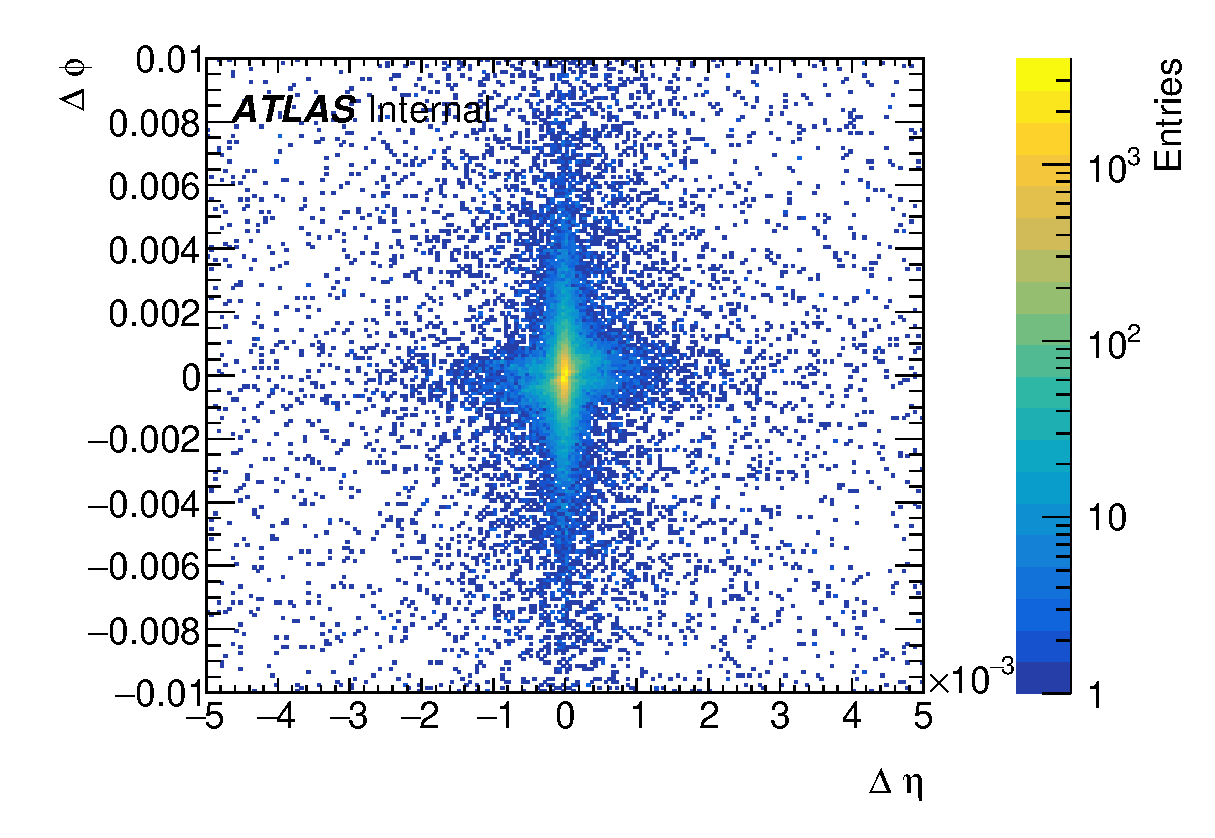
\includegraphics[width=0.55\linewidth]{images/trk_el_deta_dphi_jetsample488573.eps}
     \caption{ The correlation between the electrons of at least 'Loose' WP and 10 GeV of \pT and selected tracks of any \pT}
     \label{fig:el_trk_corr}
 \end{figure}

\blue{To be expanded.} \black{}

\green{}
\section{Spectrum unfolding}
Both spectra \pp and \OO were unfolded using the RooUnfold package \cite{Adye2011RooUnfold}. Response matrices were generated using the MC samples listed in Tables \ref{tab:pythia} and \ref{}.



\black{}

\section{Summary}
The final choice of track cuts used in the analysis is listed in Table~\ref{tab:tab_cuts}.
%{\red It'll be better to separate the d0 and z0 cuts into two lines, as we are unsure whether one shall apply both. If that is possible, move the percentiles of losses here. BTW, when you write that track, jet matching does not change the percentage; it's better that you only consider high-\pT tracks.}
\begin{table}[ht!]
  \caption{Track selection criteria in $\pprefSample$ data sample}%
  \label{tab:track_sel_pprefSample}
  \centering
  % \resizebox{\textwidth}{!}{
  \begin{tabular}{ll}
    \toprule
    Track quality    & \texttt{TightPrimary} \\
    Track-to-vertex matching criteria in $d_0$     & $|d_0| < \qty[parse-numbers=false]{1.5}{\mm}$ \\
    Track-to-vertex matching criteria in $\omega_0$     & $|\omega_0| < \qty[parse-numbers=false]{1.5}{\mm}$\\
    Significance cut on $d_0$                & $|d_0/\sigma_{d_0}| <4$ \\
    Significance cut on $\omega_0$                & $|\omega_0/\sigma_{\omega_0}| <4$ \\
    Associated vertex                & $|z_\text{vtx}| < \qty{150}{\mm}$ \\
    Track-to-jet association        & \(\mathrm{d}R < 0.4\) for $\pT>\qty{30}{\GeV}$ \\
    \bottomrule
    \label{tab:tab_cuts}
  \end{tabular}
  % }
\end{table}
The fraction of tracks selected after each cut (cutflow) in the high-$\mu$ sample is presented in Table~\ref{tab:cutflow_highmu}.
\begin{table}[h]
    \centering
    \caption{Cutflow on tracks in high-$\mu$ $\pprefSample$ sample}
    \begin{tabular}{c|c}
    Cut & Fraction after applying \\
    \hline
    Quality: ''Loose'' & $100\%$ \\
    Quality: ''TightPrimary'' & $84.9\%$ \\
    $|d_0| < 1.5$ mm & $78.5\%$ \\
    $|d_0/\sigma_{d_0}| < 4$ & $77.1\%$ \\
    $|\omega_0| < 1.5$ mm & $74.1\%$ \\
    $|\omega_0/\sigma_{\omega_0}| < 4$ & $72.1\%$ \\
    $|z_\text{vtx}| < 150$ mm & $71.2\%$ \\
    $dR<0.4$ \&\& $\pT>20$ GeV & $71.2\%$ \\
    \end{tabular}
    \label{tab:cutflow_highmu}
\end{table}
The same selection criteria will be applied in $\OOSample$ and $\NeNeSample$ samples. 

The resulting raw spectrum is presented in Figure~\ref {fig:trk_pt_cutflow}. See the performance of the cuts on different distributions in the appendix.
\begin{figure}[h]
    \centering
    \includegraphics[width=0.49\textwidth]{images/trk_pt_cutflow_.png}
        \includegraphics[width=0.49\textwidth]{images/trk_Z0_cutflow_.png}
    \caption{Cutflow of \pT (left) and $z_0$ (right) distributions in \pp data. 
    %{\red Do you understand why jet matching cuts on z that much? }
    }
    \label{fig:trk_pt_cutflow}
\end{figure}



%\begin{figure}[h]
%    \centering
%    \includegraphics[width=0.5\linewidth]{images/trk_z0_cutflow_.png}
%    \caption{Selection cutflow as a function of $z_0$}
%    \label{fig:z0_cutflow}
%\end{figure}
\chapter{Corrections}
\label{chap:corr}

\section{Trigger efficiency}
Trigger efficiency of $\pprefMBtrig$ for the $\pprefSample$ could not be determined data-driven, due to the control trigger missing on the menu and resurrection option being turned off. For the $\OO$, it will be determined using the control trigger HLT\_no\_alg\_L1\_RD0, which will be present on the menu. In Run 1, for $\pPb$ \cite{pPb_mbsptrk_trigger} the trigger efficiency $\epsilon_{\mathrm{trigger, pp}}$ for $\pprefMBtrig$ was determined to be fully efficient for events with loose track multiplicity > 2 and with $\epsilon_{\mathrm{trigger, pp}} = 99.6\pm0.3\%$ for multiplicity 2. This analysis takes these efficiencies and applies them at the closest level of quality in our selection (loosePrimary + d0).

For events with fewer tracks, there is no reference. However, events with 0 (loosePrimary + d0) tracks - making up 0.2\% of events in the studied sample - have in 99.2\% cases 0 vertices in the event, thus they do not change the $\RAA$ determination. Therefore, for events with 0 tracks, no efficiency correction is applied as it would have a negligible effect on the final spectrum.

In case of events with (loosePrimary + d0) 1 track - making up 0.7\% of events in the studied sample - there are 90 \% events with 0 vertices, and the remaining 10 \% of events have 1 vertex. Again, the overall contribution of these events to the spectrum is negligible, given the average number of vertices is 2.5 and the average number of good tracks is 66. Thus, no correction on the trigger efficiency is applied.

\section{Vertex reconstruction efficiency}
The vertex reconstruction efficiency $\epsilon_{\mathrm{vtx}}$ is determined in a data-driven approach as the ratio of triggered events with a reconstructed vertex to the total number of triggered events as a function of the number of tracks in our fiducial space using the low-$\mu$ data. The measured efficiency is plotted on Figure~\ref{fig:vrtx_eff}. Efficiency is shown for various diffraction modes based on the $\forwardgap$ cut as a function of the number of tracks in the analysis fiducial space. Inclusively, the efficiency is $\epsilon_{\mathrm{vtx}} = 95.7\%$. Since the $\RAA$ is measured using the number of vertices, this correction must be applied to every vertex. One can correct for $\epsilon_{\mathrm{vtx}}$ differentially based on $\ntrk$, when retrieving events with 1 vertex reconstructed as events with 0 vertices. However, in the case of higher $\mu$, the only option is to correct the total number of vertices in the analysis $\nvtx$. This is possible if one considers vertex reconstruction independent, and thus, its efficiency is also independent. 

\begin{figure}
    \centering
    \includegraphics[width=0.5\linewidth]{images/vrtx_eff.png}
    \caption{Vertex reconstruction efficiency}
    \label{fig:vrtx_eff}
\end{figure}


%{
%\red Found events with $0$ vertices yet some number of tracks (see fig.~\ref{fig:trkpt_novtx}). There seems to be a clear threshold at 0.4, indicating that to create a vertex, there should be a track with $p_T$ more than 0.4 GeV. Figure out how many actual collisions we miss by that (e.g., if we keep those tracks)? Monte-Carlo?

%\begin{figure}
%    \centering
%    \includegraphics[width=0.5\linewidth]{images/trkpt_novtx.png}
%    \caption{Pt of tracks with events with no vertices}
%    \label{fig:trkpt_novtx}
%\end{figure}

%}

% poisson-vertex method


\section{Pileup}
\label{sec:vertex_merging}

Due to the fact that several collisions can occur during the same bunch crossing, for a number of collisions that happen close to each other, the reconstruction algorithm may fail to resolve their vertices~\cite{ATLAS:2016nnj}. This results in two effects. The number of vertices is not properly determined. The position of the merged vertex is shifted with respect to the positions of the original vertices. Although the merging happens in 3D, the main effect is in $z$ coordinates because of the much longer $z$-dimension of the beam spot. 

One can estimate the number of merged vertices directly from the data and correct for it using the following procedure. 

Distribution of $z$-distances between all pairs of vertices is shown in the left panel of Figure~\ref{fig:vtx_z_dist}. 
\begin{figure}[h]
\centering
\includegraphics[width=0.26\textwidth]{images/vertex_z_dist_488589.png}
\includegraphics[width=0.38\textwidth]{images/fit_bw_z.png}
\includegraphics[width=0.34\textwidth]{images/fit_merg_prob.png}
\caption{Left: Distance $\Delta z^{ij}$ between vertices in chunk of run 488589, with $\langle \mu \rangle \sim 4.0$. Middle: Symmetrized distribution $|\Delta z_\text{vtx}^{ij}|$ and fit with $f(\Delta z)$. Right: Merging probability function $\mathcal{P}(\Delta z)$. 
%{\red suggest to improve the quality of these plots so that they look better in a line.}
%{\blue Can one improve plotting the function such that it does not change derivative at low values, but has it identically equal to zero? Knowing ATLAS, this curve is "an invited question". I'd avoid that.}
    \label{fig:vtx_z_dist}}
\end{figure}
The drop around zero demonstrates the effect of vertices merging. The slight asymmetry of the distribution might come from the internal ordering of the vertex coordinates. The distribution is symmetrized by taking the absolute value of the vertex distance as shown in the middle panel of the Figure. Symmetrized distribution is 
%the "dip" region ($|\Delta z^{ij}_\text{vtx}|< $ \qty{10}{\mm}) is shown in Figure~\ref{fig:vertex_dz_fit}.  
%  \begin{figure}[h]
%      \centering
%      \includegraphics[width=0.45\linewidth]{images/fit_bw_z.png}
%      \includegraphics[width=0.45\linewidth]{images/fit_merg_prob.png}
%      \caption{Left: symmetrized distribution $|\Delta z_\text{vtx}^{ij}|$ and fit with $f(\Delta z)$. Right: Merging probability function $\mathcal{P}(\Delta z)$ }
%      \label{fig:vertex_dz_fit}
%  \end{figure}
%  is fitted to the function $f_1$ and the rest with $f_2$ (see below). After such estimation of initial parameters, the total function
  \begin{equation}
      f(\Delta z) = \frac{A_1}{2\pi}\frac{\Gamma}{(\Delta z - M)^2 + \Gamma^2/4} + A_2\exp{\left(-\frac{(\Delta z - \mu)^2} {\sigma^2} \right)} = f_1(\Delta z) + f_2(\Delta z)
  \end{equation}
  %is fitted to the distribution 
  in the range $[0,70]$ mm. Extracted fit ($\chi^2/\text{n.d.f}\approx 1$) parameters are listed in Table~\ref{tab:bw_gaus_pars} 
  % {\red is that important? I think showing the fit is perfectly enough, but if you want to keep it, I suggest commenting on its stability for different values of $\mu$. This universality is rather important for the analysis, but the fit values are not so much. They would change run-by-run if the width of the \zvtx changes.} 
  \begin{table}[h]
      \centering
      \caption{Parameters of $f(\Delta z)$}
      \begin{tabular}{c|c}
           Parameter & Value  \\
           \hline
           % NOT ROUNDED
           % $A_1$ & $-58354.6 \pm 1037.83$ \\
           % $M$ & $0.531183 \pm 0.0267741$ \\
           % $\Gamma$ & $5.53881 \pm 0.0786292$ \\
           % $A_2$ & $8838.9 \pm 36.3994$ \\
           % $\mu$ & $-4.77708 \pm 1.13528$ \\
           % $\sigma$ & $85.6301 \pm 0.833025  $ \\
           % ROUNDED
           $A_1$ & $(-584\pm 10)\times10^2$ \\
           $M$ [mm] & $0.531 \pm 0.027$ \\
           $\Gamma$ [mm] & $5.54 \pm 0.08$ \\
           $A_2$ & $8839 \pm 40$ \\
           $\mu$ [mm] & $-4.8 \pm 1.1$ \\
           $\sigma$ [mm] & $85.6 \pm 0.8$ \\
      \end{tabular}
      \label{tab:bw_gaus_pars}
  \end{table}
Extracted fit parameters allow for determining the merging probability function $|f_2/f_1|(z)$ 
%{\red I found fancy $\mathcal{P}(\Delta z) = |f_1(\Delta z)/f_2(\Delta z)|$ further in the text. if you want that, please label y axis of the plot accordingly} 
that two vertices merge at a given distance in $z$. This function is shown in the right panel of Figure~\ref{fig:vtx_z_dist}.

Parameters of $z$-vertex distribution, expected to be Gaussian. 
%{\blue if you want to convince a reader that the distribution is Gaussian, put a graph in logy. people typically can say parabola by eye. I.e., the plot on the left must also be in logy.} 
They are plotted for events with $\nvtx=1$  in the left panel of Figure~\ref{fig:nvtx_ppref}. 
  \begin{figure}[h]
      \centering
      \includegraphics[width=0.45\linewidth]{images/vertex_z_488589.png}
      \includegraphics[width=0.45\linewidth]{images/nvertex_488589.png}
      \caption{Left: \zvtx distribution for events with $\nvtx=1$ in run 488589. Right: $\nvtx$ distribution in the same run.}
      \label{fig:nvtx_ppref}
  \end{figure}
The right panel of the same figure shows the number of reconstructed vertices found in the data. The $\langle \nvtx \rangle=2.96$ corresponds to $\mu\approx4$ in this run. This distribution is close to a Poisson, but it falls faster at high $\nvtx$ because the vertex merging depends on the number of collisions in a bunch crossing. 

To estimate this effect, the $\nvtx$ distribution was randomly generated assuming a Poisson shape for the number of vertices, and a Gaussian distribution in \zvtx. The width of the Gaussian is chosen the same as shown in the Figure~\ref{fig:nvtx_ppref}, and the mean value of generated vertices is slightly above the mean value in the Figure. Using the merging probability function shown in the right panel of Figure~\ref{fig:vtx_z_dist}, the number of vertices was recalculated. 
%According to this distribution, $N_\text{gen}^{\text{truth}}$ vertices are sampled. The number of vertices to be generated is sampled from a Poisson distribution with $\lambda$ taken as $\langle \nvtx \rangle=2.96$ from $\pprefSample$ data (see fig.~\ref{fig:nvtx_ppref}). 
The generated number of vertices is tuned iteratively to match the generated distribution after merging to the real data distribution up to a percent accuracy in the region of $\nvtx \leq 8$ %(see %fig.~\ref{fig:ratio_nvtx_real_over_fake}). 
The ratio of recalculated to measured $\nvtx$ is shown in Figure~\ref{fig:ratio_nvtx_real_over_fake}.
  \begin{figure}[h]
      \centering
      \includegraphics[width=0.5\linewidth]{images/nvtx_gen_real.png}
      \caption{Ratio of real $\nvtx$ distribution to $N_\text{gen}^\text{obs}$}
      \label{fig:ratio_nvtx_real_over_fake}
  \end{figure}
The region of $\nvtx > 8$ deviates from unity, however it contains less than $0.5\%$ of analyzed events.

Vertex merging was implemented in two different flavors. A simple merging algorithm orders the vertices in $z$ and merges them based on the probability explained above. The merging is performed sequentially, and when the two vertices are merged, they are replaced by a single vertex in the middle. The algorithm stops when the last vertex in $z$ is reached. A clustered merging algorithm starts with a vector of vertices, producing a binary merging decision for each pair of neighboring vertices, giving rise to a vector of boolean decisions: true or false. If there are $n$ consequential 'true' evaluations, corresponding $n$+1 vertices are merged into one located at the center of mass of these $n$+1 vertices. No significant difference was observed between these two approaches. %(see appendix, fig.~\ref{fig:ratio_seq_clus_merger}). {\red if there is no difference, I'd not invent an appendix for it}

After running the merging algorithm, the number of observed vertices is counted $N_\text{gen}^\text{obs}$. A map between the observed number $N_\text{gen}^\text{obs}$ and the truth number of vertices before merging $N_\text{gen}^\text{truth}$ is constructed shown in  Figure~\ref{fig:nobs_vs_ngen}.
  \begin{figure}[h]
      \centering
      \includegraphics[width=0.45\linewidth]{images/nobs_vs_ngen.png}
      \includegraphics[width=0.45\linewidth]{images/ratio_nobs_ngen.png}
      \caption{Left: 2D distribution of $N_\text{gen}^\text{obs}$ vs $N_\text{gen}^\text{truth}$. Right: correction factor $\varepsilon_\text{m} (N_\text{gen}^\text{obs})$}
      \label{fig:nobs_vs_ngen}
  \end{figure}
  
  For each $N_\text{gen}^\text{obs}$ $\langle N_\text{gen}^\text{truth}\rangle$ is calculated. Then, a correction factor to adjust for merging is defined as 
  \begin{equation}
      \varepsilon_\text{m}(N_\text{gen}^\text{obs}) =\langle N_\text{gen}^\text{truth}\rangle/ N_\text{gen}^\text{obs}
  \end{equation}
  The total correction factor is taken as average over $N_\text{gen}^\text{obs}$
  \begin{equation}
      \varepsilon_\text{m} = \sum_{N_\text{gen}^\text{obs}} p(N_\text{gen}^\text{obs})\varepsilon_\text{m}(N_\text{gen}^\text{obs})
  \end{equation}
and equal to 1.052 in $\langle \mu \rangle \sim 4.0$ data. {\blue To be updated -- calculated as a function of $\mu$.} 

% {\red a logical end to this section would be Figure~\ref{fig:tpvreco_bothmu}, and discussion of $N_{\mathrm{evt}}$ correction followed by the discussion of $\omega$ cuts, see my text around that figure. But to do it right, the first thing is to work out the correction not for a single $\mu$ but for any $\mu$ up to say $\mu$ of 5 and plot it as a curve.}
  
\section{Correction for track acceptance difference between 2024 and 2025 conditions}
{\blue Will be determined by comparing full-sim Pythia MCs with $\pprefSample$ and before-$\OO$ conditions.}

\section{Correction of $\avgNcoll$}
Although the \Ncoll needed for \RAA is extracted from the Glauber model, one shall take into account that the MinBias sample is not fully inclusive, and some losses are anticipated for events with low multiplicity.
{\blue Will be determined when $\OO$ data is available.}
% {\red why does one need oxygen data for that? one can do it by convolving \pp. Generally, I think this  discussion should go to \Ncoll calculations using Glauber}



\section{Correction for transmutation}\label{sec:transmutation_correction}

If oxygen dissociates into lighter nuclei with the same rigidity ($A/Z$), these lighter ions could stay circulating in the beamline together with oxygen \cite{transmutation_lpc}. The dissociation can be caused by electromagnetic dissociation or by hadronic fragmentation processes. Certain theoretical models describing oxygen as a cluster of 4 \al particles give an exceptionally high cross section to the hadronic fragmentation in \al particles, causing contamination of the \OO collisions with \Oa and \alal collisions with increasing time of the beam circulation. Such contamination (if significant enough) would inevitably affect the measurement of $\RAA$.

The approach to mitigate a possible contamination is to select the fragment of data with lower contamination levels, and by the level of contamination to increase the systematic on $\avgNcoll$ or adjust $\avgNcoll$ as a function of the contamination. Thus, one needs to be able to estimate the fraction of \Oa and \alal in the data. Assuming the average number of tracks per collision (vertex) $\tpv$ (see below) is constant, as it originates in the type of collided system and reconstruction efficiency, one can study this variable during the \OO data-taking to constrain the contamination of \OO by \Oa (\alal). One also assumes the collisions start with a pure \OO sample and the contamination builds up over time, leading to a decrease in $\tpv$, which can serve as a proxy for the contamination.


% editing stop here -> check nchar vs. ntrk in Hijing and Angantyr... we have full reco now

Using HIJING simulations for the \OO and \Oa collisions, histograms for the number of charged hadrons $\nchar$ with $|\eta|< 2.5$  and $\Npart$ were populated. Additionally, $\Npart$ and $\ntrk$ were simulated in Angantyr and Glauber. Sampling from these histograms based on the probability of the $\OO$ and $\Oa$ collisions (see below), histograms of gradually growing contamination were created. The rate of collisions of various species can be determined as: 

\begin{equation}
\begin{split}
    p_{\OO} = f_{\mathrm{O}}^{2} \sigma_{\OO} \mathcal{L}, \\
    p_{\Oa} = 2 f_{\mathrm{O}} f_{\alpha} \sigma_{\Oa} \mathcal{L}, \\
    p_{\alal} = f_{\alpha}^{2} \sigma_{\alal} \mathcal{L},
\end{split}
\end{equation}
where $f_{\mathrm{O}}$ is the fraction of oxygen nuclei in the beams, $\mathcal{L}$ the instantaneous luminosity, and $f_{\alpha}$ is the fraction of $\alpha$. Given $\alpha$ is expected to play the dominant role among the parasitic nuclei species in the \OO beam, we set for simplicity $f_{\mathrm{O}}$+$f_{\alpha} = 1$. Corresponding cross-sections $\sigma_{\OO}= (1.33\pm0.07)$~b, $\sigma_{\Oa} = (0.71\pm0.02$)~b, and $\sigma_{\alal} = (0.328\pm0.002)$~b have been obtained from the MC Glauber simulations and may have limited precision. Having these probabilities at hand, one can study the ratio of events produced in $\Oa$ and $\alal$ collisions normalized to the number of $\OO$ collisions:
\begin{eqnarray}
\frac{p_{\Oa}}{p_{\OO}} &=& 2 \frac{f_{\alpha}}{(1-f_{\alpha})} \frac{\sigma_{\mathrm{\Oa}}}{\sigma_{\mathrm{OO}}}, \nonumber \\
\frac{p_{\mathrm{\alpha\alpha}}}{p_{\mathrm{OO}}} &=& \frac{f^2_{\mathrm{\alpha}}}{(1-f_{\alpha})^2} \frac{\sigma_{\mathrm{\alpha\alpha}}}{\sigma_{\mathrm{OO}}} = 
\frac{1}{2}\frac{f_{\mathrm{\alpha}}}{(1-f_{\alpha})}
\frac{\sigma_{\alal}}{\sigma_{\alpha\mathrm{O}}}
\frac{p_{\Oa}}{p_{\OO}}.
\label{eqn:paa}
\end{eqnarray}
If the $\frac{p_{\Oa}}{p_{\OO}}$ contamination in the data stays within 20\%, the addition of \alal collisions in the data should not exceed 0.9\% using equations~\ref{eqn:paa}. Since the data collection limit is set to not exceed 10 \% $\alpha$ contamination, only $\Oa$ collisions are considered as a possible addition to \OO collisions.

Finally, the mean of the $\Npart$ and $\ntrk$ histograms was calculated. The means obtained normalized to the initial values of pure oxygen $\Npart(t=0)$ and $\ntrk(t=0)$ are shown as a function of $\frac{p_{\mathrm{\Oa}}}{p_{\mathrm{OO}}}$ in Figure~\ref{fig:corr_norm}. Normalization to the initial values is beneficial, as it removes the dependence on the detector effects. 

\begin{figure}[h]
    \centering    
    \includegraphics[width=\linewidth]{images/mixing_scan_all_observables.png}
    \caption{Average of $\Npart$ and $\ntrk$ normalized on the pure oxygen values as a function of the ratio between the probability (number) of parasitic and target events. Vertical dashed lines correspond to 5, 10, and 20 \% of $f_{\mathrm{\alpha}}$ beam contamination}
    \label{fig:corr_norm}
\end{figure}

One can see in Figure~\ref{fig:corr_norm} the difference between $\Npart$ and $\ntrk$ scaling, which requires further investigation. The difference between $\Npart$ and $\ntrk$ scaling should be considered a systematic error. Fortunately, the discrepancy is smaller for smaller values of $f_{\mathrm{\alpha}}$. Another feature of the $\Oa$ collisions is that the produced particles are boosted and $\OO$ are not. In $\OO$ HIJING used, a small asymmetry of the $\eta$ distribution of the charge particles (cut on the reconstruction and acceptance limit of the ATLAS - $\pT$ > 0.1, |$\eta$| < 2.5) was observed, as shown in Figure~\ref{fig:eta_ntrk}. This phenomenon requires further investigation. 
\begin{figure}[h]
    \centering
    \includegraphics[width=\linewidth]{images/eta_comparison.png}
    \caption{$\eta$ distribution of charged particles in HIJING $\OO$ and $\Oa$ (normalized on the integral), one can see the boosted distribution in $\Oa$ collisions and the so far not understood asymmetry in $\OO$ collisions.}
    \label{fig:eta_ntrk}
\end{figure}

Critical for the measurement in case of the transmutation is the ability to measure the $\frac{p_{\mathrm{\Oa}}}{p_{\mathrm{OO}}}$ based on the drop of the $\tpv$, which allows us to adjust $\Ncoll$ to reflect on the admixture of helium in the collision system.

For the success of the method, it is also needed to adjust for the drop of $\tpv$ originating in the dropping $\mu$, and accordingly, the $\tpv$ should not change for one collision system without the change of $\mu$. As a hint to understand the stability of the average number of tracks per vertex
$\tpv$ was considered:
\begin{equation}
  \tpv = \langle \ntrk^\text{sel}(\text{vtx}_i) \rangle,
\end{equation}
where $\ntrk^\text{sel}(\text{vtx}_i)$ is the number of selected tracks that pass the following criteria:
\begin{enumerate}
    \item Quality: TightPrimary 
    % {\red \pT, $\eta$? why shall it be different from section 4?}
    \item Matched to vertex $i$ based on cuts on $d_0$ and $\omega_0$:
    \begin{equation}
        |d_0| < \qty{1.5}{\mm}, \quad
        |\omega_0| < \qty{1.5}{\mm}, \quad
        |d_0/\sigma_{d_0}| < 4, \quad
        |\omega_0/\sigma_{\omega_0}| < 4.
    \end{equation}
\end{enumerate}
One can notice that these are the track final selections without the track-to-vertex and the track-to-jet matching criteria. $\tpv$ was studied in the $\pprefSample$ sample as a function of $\mu$, vertex position $\mathrm{z_{vtx}}$, and LB number representing the temporal dependence. See Figure~\ref{fig:highmu_lowmu_tpv} for these dependencies in high-$\mu$ and low-$\mu$ samples. 
%{\red What am I supposed to learn from these six colorful plots? A good way to decide whether you need a plot or not (and whether it is plotted correctly) is to ask yourself if you can derive any conclusion from the plot that helps the flow of convincing the reader that you are doing the right things, i.e., explaining the analysis. If not, then the plot is not needed.} Agreed, will be removed when new set of plots presented

A mild increase of $\tpv$ is seen with increasing $\mu$ (when $\mu \sim 4$), which is attributed to the effect of vertex merging (see Section~\ref{sec:vertex_merging}), since a merged vertex must have more tracks, thus moving the mean. 
%The same effect is seen on $z_\text{vtx}$ distribution ($\mu\sim 4$), where the maximum $\tpv$ is reached towards the center of the distribution, where again merging of vertices is dominant (simply because the vertex "density" there is larger).

\begin{figure}[h]
    \centering
    \includegraphics[width=0.32\linewidth]{images/tpv_lb_high_h2d_tpv_lb_488573.png}
    \includegraphics[width=0.32\linewidth]{images/tpv_mu_high_h2d_tpv_mu_488573.png}
    \includegraphics[width=0.32\linewidth]{images/tpv_zvtx_high_h2d_tpv_zvtx_488573.png}
    \includegraphics[width=0.32\linewidth]{images/tpv_lb_low_h2d_tpv_lb_488573.png}
    \includegraphics[width=0.32\linewidth]{images/tpv_mu_low_h2d_tpv_mu_488573.png}
    \includegraphics[width=0.32\linewidth]{images/tpv_zvtx_low_h2d_tpv_zvtx_488573.png}
    \caption{$\tpv$ distributions in high-$\mu$ (top row) and low-$\mu$ (bottom row) samples. Left: as a function of lumiblock number. Middle: as a function of $\mu$. Right: as a function of $z_\text{vtx}$.}
    \label{fig:highmu_lowmu_tpv}
\end{figure}

As $\OO$ mean $\mu$ is expected to be low ($\sim 0.3$), the $\tpv$ dependencies in $\pprefSample$ low-$\mu$ sample can be taken as reference. Less granular quantities can be defined
\begin{equation}
    \avgtpvreco = \frac{N_\text{trk}^\text{reco}}{N_\text{vtx}}, \quad 
    \avgtpvsel = \frac{N_\text{trk}^\text{sel}}{N_\text{vtx}}, \quad 
\end{equation}
where subscript $\text{reco}$ refers to reconstructed tracks (no selections applied) and $\text{sel}$ subscript refers to tracks selected as ''TightPrimary'' \&\& $|d_0|<\qty{1.5}{\mm}$ \&\& $|d_0/\sigma_{d_0}|<4$. 
%{\red already explained. when you repeat things in the text, you make them less certain to a reader. much better way is to define tracks once and always use the same tracks.} This is done here to emphasize not using omega0 cut... Will be reiterated
They are equivalent to $\tpv$ in the regime of low-$\mu$, as then $\nvtx \sim 1$. As can be seen from Figure~\ref{fig:tpvreco_bothmu}

% {\red Figure~\ref{fig:tpvreco_bothmu} belongs to the end of section 5.3, and it has to have 3 curves. To put them on one canvas, one can rebin $\mu$ intervals at the edges such that the error bars are not too large there, or just ignore points with error bars greater than 1/2 track (must be mentioned in the captions). 

% The first curve must be as shown. 

% The second curve must be after applying the correction explained in section 5.3. The anticipated effect is that the left interval will stay where it is, but the right interval will go significantly down, I would expect below 24-25 tracks. The correction must be applied differently for each value of $\mu$. 

% The third curve also must have the correction applied for vertex merging, but it should have a different track selection with $\omega$ cuts. For example, the first set of cuts should assign any track to the nearest vertex regardless of $\omega$, and the other set of cuts should use the full suite of $\omega$-based selection. The anticipated effect of the third curve is that it may go up or down depending on which set you use originally, but both $\mu$ intervals would become flat.

% Using the figure, we must make a conclusion that merging move vertices and invalidating the $\omega$ cuts, and deciding whether we shall or shall not use them at all. In here, you can simply refer to that plot in section 5.3}

% This will be added in the next version



\begin{figure}[h]
    \centering
    \includegraphics[width=1.0\linewidth]{images/TPVreco_bothmu.png}
    \caption{Dependence of $\langle \avgtpvreco \rangle$ on $\mu$ in chunk of $\pprefSample$ sample ($\langle \mu \rangle\sim 0.2$ and $\langle \mu\rangle\sim 4.0$)}
    \label{fig:tpvreco_bothmu}
\end{figure}
the quantity $\langle \avgtpvreco \rangle$ is constant in the regime of low-$\mu$, and is rising for high-$\mu$ (due to effect of merged vertices). 


%Distributions of $\tpv$ as a functions of lumiblock, $\mu$ and $z_\text{vtx}$ were fitted with pol1. Resulting slopes are consistent with 0 within $2\sigma$ with $\chi^2/\text{ndf}\sim 1$. Dependence on $z_\text{vtx}$ still have certain degree of a non-constant behavior in range $|z_\text{vtx}| > \qty{100}{\mm}$
% \begin{figure}[h]
%     \centering
%     \includegraphics[width=0.32\linewidth]{images/meantpv_lowmu_lb.png}
%     \includegraphics[width=0.32\linewidth]{images/meantpv_lowmu_mu.png}
%     \includegraphics[width=0.32\linewidth]{images/meantpv_lowmu_zvtx.png}
%     \caption{Mean $\tpv$ in low-$\mu$ sample. Left: as a function of lumiblock number. Middle: as a function of $\mu$. Right: as a function of $z_\text{vtx}$}
%     \label{fig:lowmu_mean_tpv}
% \end{figure}
\chapter{Glauber modeling}\label{chap:glauber}

\section{$\avgNcoll$ for minimum bias collisions}\label{sec:ncoll_glauber}
The present $\RAA$ measurement is performed without centrality differentiation, i.e., integrated over the available impact parameter $b$ range. Calculation of $\avgNcoll$ is performed in the Monte-Carlo Glauber (MCG) approach using publicly available code of TGlauberMC \cite{alver2008phobosglaubermontecarlo, PhysRevC.97.054910}.

There are several input parameters to TGlauberMC:
\begin{enumerate}
    \item Inelastic nucleon-nucleon cross-section $\sigma_{_\mathrm{NN}}$. For $\sqn = \qty{5.36}{\tev}$ it is taken as $\sigma_{_\mathrm{NN}}= \sigma_{\pp} =~68.2\pm~\qty{0.6}{mb}$ from \cite{PhysRevC.97.054910} as linear interpolation between 5.02 and 5.44 TeV
    \item Minimal distance between nucleons $d_\text{min}$ with a default value of $d_\text{min} = \qty{0.4}{fm}$ %In the improved version, a space lattice is introduced with separation $d_\text{node}$
    \item Geometric model of colliding nuclei. Three models for oxygen are available (in TGlauberMC): harmonic-oscillator model, Woods-Saxon parametrization (3-parameter Fermi, 3pF), and a model based on direct wave-function calculation. For neon 3pF parametrization was implemented with parameters taken from \cite{DEVRIES1987495}
    % \item Nucleon collision profile
    % \begin{equation}
    %     P(b_{NN}) = \Gamma \left(1/\omega, b_{NN}/D^2\omega \right) / \Gamma (1/\omega)
    % \end{equation}
    % with parameter $\omega$, with $\omega=0$ reducing to "black-disk" approximation, and with $\omega=1$ to Gaussian profile. Value of $\omega=0.4$ is quoted to reproduce $\pp$ cross-sections at LHC energies \cite{PhysRevC.97.054910}, and therefore is taken as default
    % \item Event-by-event fluctuations of $\sigma_{NN}$ (color fluctuations inside nucleons):
    % \begin{equation}
    %     P_\sigma(\sigma_{NN}) = C \frac{\sigma_{NN}}{\sigma_{NN} + \sigma_0}\exp{\left(-\left[\frac{\sigma_{NN}-\sigma_0}{\sigma_0\Omega}\right]^2\right)}
    % \end{equation}
\end{enumerate}

Resulting distributions of $\Ncoll$ and $\Npart$ for $\OO$ calculated in TGlauberMC (with two different geometry models) and for $\NeNe$ are presented in Figure~\ref{fig:ncoll_npart_oo}
\begin{figure}[h]
    \centering
    \includegraphics[width=0.49\linewidth]{images/NcollOO.png}
    \includegraphics[width=0.49\linewidth]{images/NpartOO.png}
    \includegraphics[width=0.49\linewidth]{images/NcollNeNe.png}
    \includegraphics[width=0.49\linewidth]{images/NpartNeNe.png}
    \caption{Top: distributions of $\Ncoll$ and $\Npart$ in $\OO$. Bottom: distributions of $\Ncoll$ and $\Npart$ in $\NeNe$}
    \label{fig:ncoll_npart_oo}
\end{figure}

\chapter{Systematic uncertainties}\label{chap:systematics}
\section{Trigger efficiency}
Systematics on the trigger efficiency changes with the multiplicity. Given that the efficiency was determined \cite{pPb_mbsptrk_trigger} using a detector under different conditions and for a different collision system, we assign to the efficiency $\epsilon_{\mathrm{trigger, pp}}$ for (loosePrimary + d0) track multiplicity == 2 absolute systematic uncertainty of 0.5~\%, for (loosePrimary + d0) track multiplicity > 2 \&\& < 5 an absolute systematic uncertainty of 0.1~\% and for multiplicity > 5 no systematic uncertainty. In the case of less than 2 tracks, no correction for the trigger efficiency was applied as these cases contribute negligibly to the $\RAA$.

\begin{comment}
\section{Vertex reconstruction efficiency}
Removing the beam background was not applied to determine the vertex reconstruction efficiency, which would likely lead to a sub-\% systematic effect based on \cite{chargedHadroninPP2010}. Major systematic errors probably arise from the assumption that the vertex reconstruction efficiency can be taken independently in events with multiple vertices. For this reason, we assign a rather safe 1\% absolute systematic till Pythia studies can be run. 

\section{Vertex merging correction factor}
The toy Monte-Carlo model described in Section~\ref{sec:vertex_merging} has several input parameters which generate systematic uncertainty on $\varepsilon_\text{m}$. The sources of systematics are the following:
\begin{enumerate}
    \item Poisson distribution parameter $\lambda$ of truth-level distribution of $\nvtx$, which taken from data and tuned iteratively. The model shows that for a chosen value of $\lambda$, the mean of the observed distribution drops by approximately 0.2 (compared to the truth). This value varies around the initial parameter. The model is rerun with $\lambda\pm0.2$ and the maximum of relative (to central value) deviation is plotted. The error is estimated from a constant function fit to the relative deviations distribution (see Figure~\ref{fig:sys_eps_m_nvtx}) and quoted as $0.4\%$.
    \begin{figure}[h]
        \centering
        \includegraphics[width=0.5\linewidth]{images/sys_unc_mean_vtx.png}
        \caption{Systematic Uncertainty of $\varepsilon_\text{m}$ for variations of $\lambda$}
        \label{fig:sys_eps_m_nvtx}
    \end{figure}
    \item The relative normalization of functions $f_1$ and $f_2$ (Section~\ref{sec:vertex_merging}), which is extracted from the fit to real data. Choice of the normalization drives the merging probability for very small $\Delta z$. To estimate the effect of the normalization parametrization, the $A_1$ parameter of $f_1$ extracted from the fit is varied up and down according to its uncertainty. The result is shown on the left of Figure~\ref{fig:sys_eps_m_bw_amp}. The parameter $\Gamma$ defines the "effective" merging region for vertices and varies within its uncertainty (the right side of Figure~\ref{fig:sys_eps_m_bw_amp}). Resulting uncertainties are $0.1\%$ and $0.05\%$.
    \begin{figure}[h]
        \centering
        \includegraphics[width=0.48\linewidth]{images/sys_unc_dg_amplitude1.png}
        \hskip10pt
        \includegraphics[width=0.48\linewidth]{images/sys_unc_dg_sigma1.png}
        \caption{Systematic Uncertainty of $\varepsilon_\text{m}$ for variations of $A_1$ (left) and $\Gamma$ (right)}
        \label{fig:sys_eps_m_bw_amp}
    \end{figure}
    \item The width of the $\zvtx$ distribution for a single vertex. The generated distribution is about $1.3\%$ wider after merging. The effect of varying the input width of $\zvtx$ by this amount results in $0.1\%$ systematic (Figure~\ref{fig:sys_eps_m_zvtx}).
    \begin{figure}[h]
        \centering
        \includegraphics[width=0.5\linewidth]{images/sys_unc_z_vtx_sigma.png}
        \caption{Systematic Uncertainty of $\varepsilon_\text{m}$ for variations of width of $\zvtx$}
        \label{fig:sys_eps_m_zvtx}
    \end{figure}
    \item The algorithm used for merging vertices. Two of the proposed algorithms were compared and are consistent throughout the whole $N_\text{gen}^\text{obs}$ range, no systematic effect is visible. No systematic uncertainty is assigned due to this choice.
\end{enumerate}
The total systematic uncertainty is calculated as the quadratic sum of these sources and equals $0.4\%$. % 0.43 to be precise
\end{comment}
\section{Luminosity of $\pprefSample$}
The luminosity of $\pprefSample$ was determined centrally it bring an uncertainty of $\delta \mathcal{L}_{pp}$ = ? \%. \blue{} Will be delivered to us by the Lumi Group. \black{}.

\begin{comment}
% commented out since the <TAA> is obtained globally

\section{Glauber modeling -- $\avgNcoll$}
Calculation of $\avgNcoll$ within the Glauber model is associated with the following systematic uncertainties:
\begin{enumerate}
    \item Underlying geometric model of nuclei. Two models for $\OO$ were used, 3pF and Wave-function (Section~\ref{sec:ncoll_glauber}). While keeping all other parameters fixed, the change in the model choice yields a difference of $3.5\%$ in the resulting $\avgNcoll$.
    \item Uncertainty of parameters of 3pF. Each parameter was varied within its known uncertainties from \cite{DEVRIES1987495}
    \item Uncertainty of inelastic cross section $\sigma_{NN}$. It was varied up and down within $\pm\qty{0.6}{mb}$ (Section~\ref{sec:ncoll_glauber})
    \item Minimal distance between nucleons $d_\text{min}$. If a given nucleon is sampled "too close" to another nucleon, its position is resampled, which introduces bias in the generated geometry. Uncertainty due to choice of this parameter is calculated by varying $d_\text{min}$ from 0.0 to 0.8 fm \cite{PhysRevC.97.054910}
    % \item Nucleon profile parameter $\omega$. It was varied up and down by $0.1$ to propagate uncertainty to $\avgNcoll$
\end{enumerate}
Each parameter was varied around its central value, and the average of absolute deviations is quoted as systematic uncertainty for a given source (Figure~\ref{fig:systematics_ncoll_oo_nene})
\begin{figure}[h]
    \centering
    \includegraphics[width=0.8\linewidth]{images/ncoll_sensitivity_OO.png}
    \includegraphics[width=0.8\linewidth]{images/ncoll_sensitivity_NeNe.png}
    \caption{Top: summary of systematic uncertainties for $\OO$ (except geometry model). Bottom: summary for $\NeNe$}
    \label{fig:systematics_ncoll_oo_nene}
\end{figure}
After summing up the geometry choice and the parameter variation systematics, the uncertainty on $\avgNcoll$ reaches $4.3\%$ for O.
\end{comment}

\section{Contamination of $\Oa$ and $\alal$}
There are three sources of systematic on correction for the $\OO$ contamination by $\Oa$ and $\alal$ collisions:
\begin{enumerate}
    \item The model dependence of $\Npart$ or $\tpv$, where the Glauber, Hijing, and Angantyr models were studied along with modifications originating in previously published measurements. The difference in their scaling, observed in Fig~\ref{fig:corr_norm}, is also a source of uncertainty. 
    \item Other uncertainty is associated with the fact that collisions will run for a certain amount of time, i.e., the transmutation will start, before the data-taking status is declared at the ATLAS detector.
\end{enumerate}


%As the left part of the fig \ref{fig:ntrk_ncoll_norm} shows, the systematic on $\avgNcoll$ grows almost linearly with the uncertainty on $\langle \tpv \rangle$, which then needs to be determined. 


% Tracks used to calculate $\tpv$ are selected with a set of cuts, which assume track-to-vertex association. To eliminate dependence on cuts, one can define similar quantities (which are just averages over a given event record)
% \begin{equation}
%     \avgtpvreco = \frac{N_\text{trk}^\text{reco}}{N_\text{vtx}}, \quad 
%     \avgtpvsel = \frac{N_\text{trk}^\text{sel}}{N_\text{vtx}}, \quad 
% \end{equation}
% for any given event and compare them {\red (stability of $\avgtpvreco$ is also ''known'', its flat within $2\sigma$)}. Given that these quantities do not depend on $\mu$ in the limit of small $\mu$ ($\sim 0.2$, see sec.~\ref{sec:transmutation_correction}), they should also be constant (in time) in the absence of contamination, which is the case for $\pp$ collisions. To quantify the systematic uncertainty related to choosing some cuts over not using them at all, the ratio $\avgtpvsel/\avgtpvreco$ is constructed. Its RMS around the mean value across the available $\pprefSample$ low-$\mu$ sample is quoted as the systematic uncertainty of $0.2\%$ (see fig.~\ref{fig:tpv_sys_lowmu_highmu}).
% \begin{figure}[h]
%     \centering
%     \includegraphics[width=0.45\linewidth]{images/tpvsel_tpvreco_lowmu.png}
%     \includegraphics[width=0.45\linewidth]{images/tpvsel_tpvreco_highmu.png}
%     \caption{Ratios of $\avgtpvsel/\avgtpvreco$ for LB where $\mu\sim\text{const}$. Left: $\langle \mu\rangle\sim 0.2$. Right: $\langle \mu \rangle \sim 4.0$}
%     \label{fig:tpv_sys_lowmu_highmu}
% \end{figure}

%The ratio of $\tpv(t_1)$ at any given time to $\tpv(0)$ (representing start of the run where no contamination is present) should be equivalent to same ratio from MC (e.g. HIJING), as all the efficiencies and corrections cancel, if we assume conditions to be constant throughout the run. The same argument applies to $\avgtpv$. Therefore, to quantify conservatively the effect of choosing cuts for $\tpv,$ one can plot the above-mentioneded ratios as a function of time (lumiblock) and compare them ({\red e.g., fit absolute deviations with a constant function and quote it as systematic})

\section{Vertex counting in the \OO sample}
Cleaning the \OO sample produces a systematic error based on the values of $\lukesvar$. {\blue Will be determined.} \black{}

\section{Difference in conditions}
{\blue Will be determined from a comparison of Angantyr with different conditions} \black{}

\section{Track momentum resolution} 
{\blue Will be determined by taking a ration between smeared $\pprefSample$ and \OO spectra.} \black{}

\section{High-\pT leptons removal} 
{\blue Will be determined.} \black{}

%\section{Gap cut} 
%{\blue Will be determined when MC Pythia samples for various diffraction modes are available, based on variations of the cut value and the mismatch of the inclusive MC on the data $\forwardgap$ distributions.}


\chapter{Results}
\label{chap:results}
{\red needs update to newest plot... Maybe add whatever we have at the moment on \RAA}

One can compare measured \RAA with the theory predictions \cite{RAA_prediction}. Values shown in the Figure~\ref{fig:RAA_prediction} were extracted by a 'data thief' and interpolated linearly between \sqn = 5.02 and 7.0 TeV. The analysis team is in contact with the authors of this paper to obtain the precise values of the suppression prediction done for \sqn = 5.02 TeV and the prediction for the no-quenching baseline. We have also requested the \pT range to be lowered below 10 GeV in the recalculation to \sqn = 5.36 TeV. Moreover, at least for the no-quenching baseline, authors of \cite{RAA_prediction_6p8} explicitly claim that the baseline is the same for \OO and \NeNe, which should be enough to put measured \RAA into a context. The theory group around Aleksas Mazeliauskas has also provided us with such a preliminary no-quenching prediction in the expected kinematic reach, shown in the Figure~\ref{fig:RAA_no_quench}. 

\begin{figure}[h]
    \centering
    \includegraphics[width=0.7\linewidth]{images/RAA_prediction.png}
    \caption{\RAA prediction based on \cite{RAA_prediction}.}
    \label{fig:RAA_prediction}
\end{figure}

\begin{figure}[h]
    \centering
    \includegraphics[width=0.7\linewidth]{images/plot_LHC_hadron_OO_RAA_90.pdf}
    \caption{No-quenching \RAA prediction valid both for \OO and \NeNe}
    \label{fig:RAA_no_quench}
\end{figure}
\input{text/Conclusions}

% All figures and tables should appear before the summary and conclusion.
% The package placeins provides the macro \FloatBarrier to achieve this.
% \FloatBarrier

%-------------------------------------------------------------------------------
% If you use biblatex and either biber or bibtex to process the bibliography
% just say \printbibliography here.
\printbibliography
% If you want to use the traditional BibTeX you need to use the syntax below.
% \bibliographystyle{obsolete/bst/atlasBibStyleWithTitle}
% \bibliography{ANA-HION-2025-03-INT1,bib/ATLAS,bib/CMS,bib/ConfNotes,bib/PubNotes}
%-------------------------------------------------------------------------------

%-------------------------------------------------------------------------------
% Print the list of contributors to the analysis.
% The argument gives the fraction of the text width used for the names.
%-------------------------------------------------------------------------------
\clearpage
\PrintAtlasContribute{0.30}
\begin{itemize}
\item Patrik Novotny: Data analysis, triggers, event selection. Text editing. 
\item Pavel Pavzderin: Data analysis, track selection. Text editing. 
\item Alexander Milov: Analysis supervision, \OO cleaning, and text editing.
\end{itemize}

%-------------------------------------------------------------------------------
\clearpage
\appendix
\part*{Appendices}
\addcontentsline{toc}{part}{Appendices}
The JER curves used in \pprefSample and \OO are shown in Figure~\ref{fig:app_jer_pp_oo}.
\begin{figure}
    \centering
    \includegraphics[width=0.45\linewidth]{images/jer_pp_v1.png}
    \includegraphics[width=0.45\linewidth]{images/jer_fits_oo_v1.png}
    \caption{JER as a function of jet \pt in \pprefSample (left) and in \OO (right)}
    \label{fig:app_jer_pp_oo}
\end{figure}
They are parametrized as 
\begin{equation}
    \text{JER}(\pt) =  \sqrt{\left(\frac{c_1}{\pt} \right)^2  + \left(\frac{c_2}{\sqrt{\pt}} \right)^2 + c_3^2 }
\end{equation}
and were worked out by HI jet group.

Track momentum resolution is obtained as follows. The distribution of $(\pt^\text{reco} - \pt^\text{gen})/\pt^\text{gen}$ is obtained in MC for different $\eta$ bins as a function of $\pt^\text{reco}$. Then for each $\eta$ and $\pt^\text{reco}$ bin the distribution is fitted with gaussian around 0 (see Figure~\ref{fig:tmr_slice}). 
\begin{figure}
    \centering
    \includegraphics[width=0.5\linewidth]{images/tmr_abs_eta1_ptreco6.png}
    \caption{Distribution of $(\pt^\text{reco} - \pt^\text{gen})/\pt^\text{gen}$}
    \label{fig:tmr_slice}
\end{figure}
The width of the gaussian is taken as TMR. TMR as a function of $\pt^\text{reco}$ is fitted with linear function of the form
\begin{equation}
   \text{TMR}(\pT) = p_0 +  p_1 \pT 
\end{equation}
which is displayed in Figure~\ref{fig:tmr_abs_all}
\begin{figure}
    \centering
    \includegraphics[width=0.6\linewidth]{images/tmr_abs_all.png}
    \caption{TMR as a function of $\pt^\text{reco}$}
    \label{fig:tmr_abs_all}
\end{figure}

% Parameters of the fit $p_0$ and $p_0$ are listed in Table~\ref{tab:tmr_par_pp} ({\red update when all JZ available and merged})
% \begin{table}
%     \centering
%     \begin{tabular}{c|c}
%        0.0146  &  0.0187 \\
%        0.000179  &  0.000291 & 
%     \end{tabular}
%     \caption{Caption}
%     \label{tab:tmr_par_pp}
% \end{table}

%-------------------------------------------------------------------------------
\end{document}
